%# -*- coding: utf-8-unix -*-
% !TEX program = xelatex
% !TEX root = ../thesis.tex
% !TEX encoding = UTF-8 Unicode

\chapter{国内外相关研究综述}
\label{chap:rw}


本章中,我们将围绕具体任务,介绍实体、关系、问句语义理解的基础知识和研究综述。
实体理解部分,我们从传统的实体链接任务出发,介绍在文本和表格中的特征工程和深度学习模型,
以及用于跨语言实体链接任务中的跨语言词向量模型;
关系理解部分,我们关注知识库补全任务,并介绍两类主要的模型,分别是规则推导模型和知识库向量模型;
问句理解部分,我们将注意力放在面向客观事实类问题的知识库自动问答任务,
同样介绍两类模型,即基于语义解析和基于信息抽取的模型,前者与我们的研究更加密切,
本节也会重点阐述语义解析模型的多个组成部分。

%# -*- coding: utf-8-unix -*-
% !TEX program = xelatex
% !TEX root = ../thesis.tex
% !TEX encoding = UTF-8 Unicode

\section{实体理解:实体链接任务}
\label{sec:rw-linking}


实体链接任务是一类从自然语言文本中识别出代表实体的字符串,
并将其映射到知识库中特定实体的任务。
人工进行的实体链接体现在维基百科的页面编辑过程中,
页面作者会手动为部分代表实体的短语添加超链接,
指向对应实体的维基页面。
这种带有维基内部超链接的短语被称为锚文本(Anchor Text),
本文中也称为实体短语。
基于机器学习的实体链接可以应用于不同场合的文本输入,
背后所使用的目标知识库也不局限于维基百科,
其它常用的知识库包括DBPedia,Yago以及Freebase。
考虑到这些知识库均基于维基百科信息构建而成,
实体链接任务又被称为``{维基化}'' (Wikification)
\cite{mihalcea2007wikify}。

以英文维基百科为例,一个典型的实体链接任务见下例:

\vspace{0.2cm}
%\begin{minipage}{0.5\columnwidth}
%\begin{center}
\underline{Michael Jordan}, also known by his initials, MJ, 
is a former professional \underline{basketball}
player. He played 15 seasons in the 
\underline{National Basketball Association} for 
the \underline{Chicago Bulls}
and \underline{Washington Wizards}.
%\end{center}
%\end{minipage}
\vspace{0.2cm}

实体链接任务首先需要提取出句中存在的实体短语,即下划线对应的部分。
该步骤与命名实体识别任务类似,
不同之处在于我们关注的实体短语除了命名实体
(具体的人名、地名、组织名、书名、电影名等)之外,
还包含了维基百科中存在的概念实体,用于指代一组相似实体。%例如森林、哺乳动物、运动员等。
下一个步骤对每个实体短语从维基百科中抽取出候选实体集,
并定义短语和候选实体之间的匹配分数,从而将短语链接至最相关的候选实体,
例如句中的5个实体短语分别对应维基百科中的实体
\textit{Michael Jordan}\footnote{https://en.wikipedia.org/wiki/Michael\_Jordan},
\textit{basketball}\footnote{https://en.wikipedia.org/wiki/Basketball},
\textit{National Basketball Association}\footnote{https://en.wikipedia.org/wiki/National\_Basketball\_Association},
\textit{Chicago Bulls}\footnote{https://en.wikipedia.org/wiki/Chicago\_Bulls}
以及\textit{Washington Wizards}\footnote{https://en.wikipedia.org/wiki/Washington\_Wizards}。

除了无结构的纯文本以外,互联网语料中的表格也蕴含了大量与实体相关的知识。
对表格进行实体链接的研究起源于Limaye等人\cite{limaye2010annotating}的工作,
如\figref{fig:rw-linking-limaye}所示,除了每个单元格所对应的实体之外,
得益于半结构化的组织形式,同一表列内的实体通常具有相同的类型,
而且两列实体之间描述了同一种关系的不同实例,
这些是非结构化文本所不具备的优势。
因为表格带来了丰富关系知识,表格上的实体链接在近年来受到了更多的关注。

\begin{figure}[th]
	\centering
    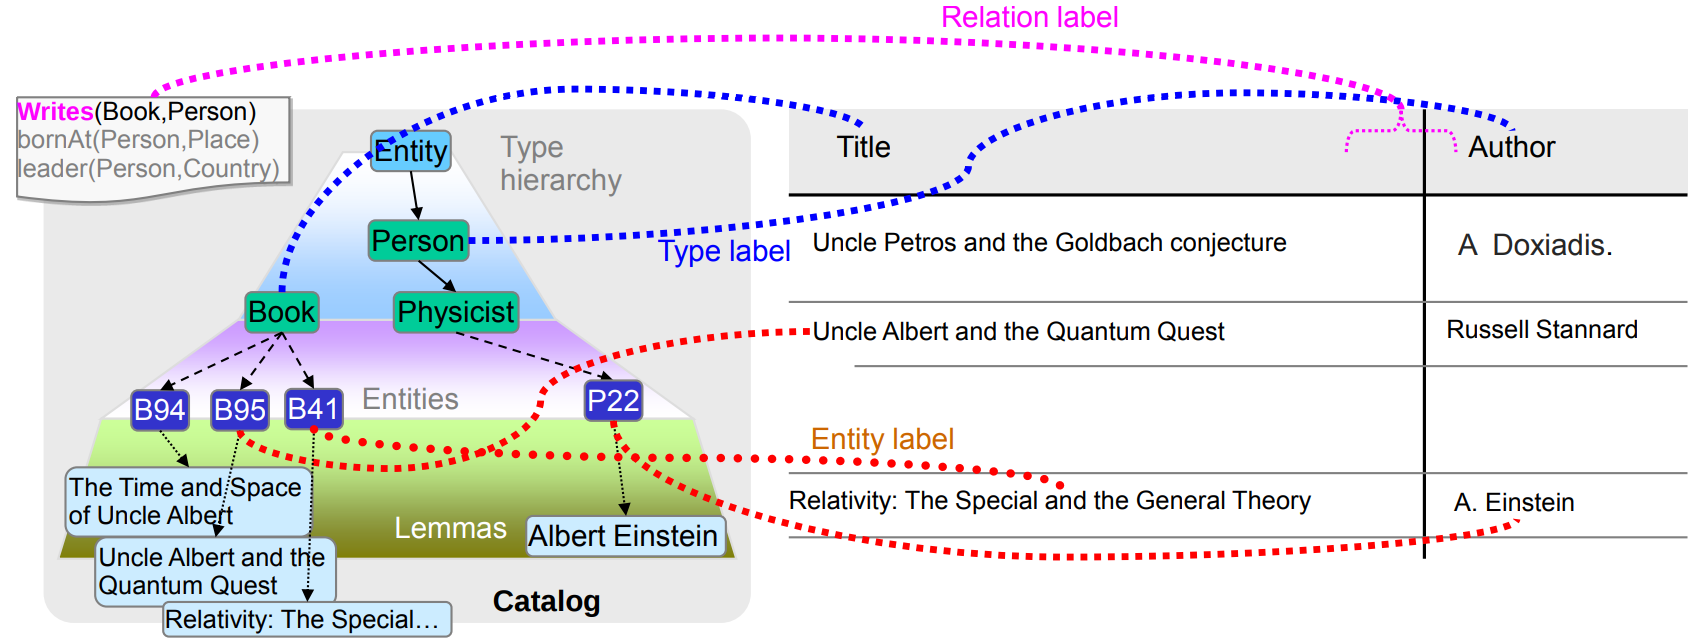
\includegraphics[width=0.95\columnwidth]{figure/rw/linking-limaye.png}
	\bicaption{Limaye等人提出的表格链接任务。\cite{limaye2010annotating}}{Entity linking task on web tables proposed by Limaye et al.}
	\label{fig:rw-linking-limaye}
\end{figure}

%讲一下和下游任务的联系,分别列举,从Han的变来
作为自然语言理解中的基本任务,实体链接是一系列下游任务的前置步骤。
%例如关系分类、阅读理解以及自动问答,
%(加上引用,有了论文就知道怎么聊)
%=============%
首先,开放式信息抽取抽取的主谓宾三元组均为文本表示,通常具有歧义,
一些研究工作旨在对三元组中的实体短语进行链接,
代表文献包括\parencite{nakashole2012patty,lin2012entity},
在实现三元组消歧的同时,结合知识库推理出主语和宾语所代表的类型,
有助于挖掘不同谓词关系之间的语义联系。
%=============%
其次,实体链接与知识库补全任务密切相关,
%带链接的关系三元组与知识库补全任务密切相关,
该任务的目的是向已有知识库中补充新的事实三元组。
这些新添加的三元组主要来源于两方面:
随时间发展所产生的全新事实,或基于已有知识的归纳推理。
基于前者的补全依赖于信息抽取系统的不断挖掘,
因此对主宾语的链接的准确率决定了知识库补全的效果。
知识库补全的相关内容将在\secref{sec:rw-kbc}中论述。
%=============%
最后,对于自动问答任务,%此处加cite?
尤其是我们关注的基于知识库的事实类自动问答任务,
其描述的是与问句中实体相关的事实,
因此不管以何种方式对答案进行建模,都依赖于对已有实体的准确定位,
以限定问句对应语义的搜索范围。
%=============%
%Information Retrieval以及Context Analysis
%都是非常重要的子任务
%实体链接结果给句子提供了知识库维度上的特征,
%并且限定整句的语义范围。
因此,实体链接的结果好坏,对这些任务的效果均有着很大程度的影响。
%常用的数据集包括xxxxx,以及表格数据集xxx

%以下是实体链接任务中的主要数据集。
%TAC-KBP\cite{}是xxxx,包含了xxxx的xxxx。
%AIDA数据集\cite{}由Hoffart等人提出,包含了。。。。
%Web Manual数据集\cite{}
%此外还有相关语料库,例如FACC1\cite{}...
%数据集:(Tutorial71-77)

实体链接的重点在于从多个候选中找出正确的那个实体,
其本质为消除实体级别存在的一词多义性,
例如短语 ``Michael Jordan'' 具有多个可能的候选,
在维基百科中可能代表篮球明星、足球运动员、著名的机器学习教授,
甚至更多不那么有名的人。
在缺乏上下文信息的情况下,很难进行准确的链接。
因此,一个良好的实体链接模型,相关性分数需要考虑多个因素,
包括实体本身的先验知识,实体与短语的匹配程度,以及实体与短语所在上下文的契合度。

基于特征工程的方式,其信息来源主要为维基百科上的统计数据。
随着深度学习的发展,
实体链接的研究将重心放在用表示学习替代或改良传统的特征工程方法。
得益于也文本的向量表示技术,以及神经网络的特征学习能力,
深度学习方法通过计算文本、实体的向量作为其语义表达,
并利用高维空间的相似度衡量短语和候选实体之间的相关性,
在效果上也取得了不错的提升。
接下来的几个小节主要介绍基于特征工程和深度学习的实体链接模型,
并单独介绍用于跨语言链接场景中的跨语言词向量技术。


\subsection{基于特征工程的实体链接}
\label{sec:rw-linking-feature}

基于特征工程的实体链接方法,较为经典的工作包括文献
\parencite{hoffart2011robust,ratinov2011local,shen2012linden,yang2015s,luo2015joint}。
这类方法的共性在于用预定义好的函数或概率值,
描述候选实体与实体短语及其上下文之间的特征,
通过学习特征的带权相加计算最终的匹配度。


在这类方法中,一个候选实体所具有的特征可以分为三类:
先验特征,上下文语义特征,以及与句中其它实体的关联特征。
%=======================%
先验特征与短语所处的文本无关,
仅基于短语与候选实体在维基百科中的统计信息,
主要体现为短语所在锚文本链接至该实体的概率,
以及实体出现在不同维基页面中的概率。
%=======================%
上下文语义特征关注文本及目标实体的语义近似程度,
利用词袋模型(Bag-of-Words)将短语的上下文
以及目标实体的维基页面分别转化为向量形式,
通过TF-IDF得到不同词语的重要性,
并用向量间的相似度
%(余弦相似度,点积或KL散度)
代表语义匹配程度。
%=======================%
实体间的关联特征体现在不同短语所对应的实体之间,
它们维基百科页面的相关性有助于实体链接的判断。
在维基百科中,若两个实体同时指向的页面较多,
或同时指向这两个实体页面的其它实体较多,
则它们具有较高的相关度。
常用的计算方式主要为点对点互信息(PMI)\cite{ratinov2011local}
或基于谷歌距离的维基链接度量(WLM)\cite{shen2012linden}。
其它的可选方式包括Jaccard相似度,以及具有非对称形式的条件概率。

对于实体链接模型的训练方式,若不同的实体短语之间互相独立,
那么训练过程是一个简单的监督学习问题,
即判断每一个\textless 短语,实体 \textgreater 对的正确性。
考虑到每个短语仅对应唯一的正样本,其余所有候选实体均为负样本,
为了保持正负样本的平衡,
一般采用Ranking SVM\cite{joachims2002optimizing}
或最大间隔(Max Margin)模型进行训练。
这样的做法称为局部优化,
显然忽略了候选实体之间的关联。
为了能捕捉这一特征,%以寻找实体链接的全局最优解(或近似最优解),
Ratinov等人\cite{ratinov2011local}首先利用局部优化方案,
对每个实体短语进行链接,得到具有一定质量的次优解,
然后根据次优解计算候选实体与其它实体的关联特征,用于完整的模型训练。
Shen等人\cite{shen2012linden}对两个实体之间的相关度计算进行了类似的简化,
将单个实体与其余短语的所有候选分别进行相关度计算,并选取最大值作为特征。
Bhagavatula等人\cite{bhagavatula2015tabel}通过迭代的方式
不断对每个短语预测的实体进行更改,
实体间的相关度特征也随着不断变化,更加靠近真实情况。
以上这些方法通过简化特征或迭代预测的方式,
使得训练过程得以保持对每一个\textless 短语,实体 \textgreater 进行打分的形式。

与之相对的全局优化方法则将整个文本以及所有不同短语的候选实体
整合在一个目标函数中,因此可以对更加复杂的相关性进行建模。
Hoffart等人\cite{hoffart2011robust}在模型中构建了一个包含所有实体短语
以及候选实体的无向图,不同的特征值体现为图中具有不同权重的边,
该模型通过贪心算法寻找图中具有最大权重的稠密子图,
使得每一个短语在子图中与唯一的一个实体相连。
Luo等人\cite{luo2015joint}利用条件随机场(CRF)
对实体链接与命名实体识别任务(NER)同时建模,
使实体链接过程能够利用NER的一系列特征。
Yang等人\cite{yang2015s}提出的S-MART模型
考虑到了多个实体短语不能重叠的限制,属于全局优化的范畴,
利用前向后向算法对所有短语进行链接,
保证在多个短语重叠的情况下,最多一个短语指向具体的实体,其余均指向空实体。
同时,该模型通过迭代决策树(MART,即GBDT)对匹配度进行建模,
MART在工业界被广泛使用,具有非常良好的效果。


\subsection{基于深度学习的实体链接}

传统的特征工程方法需要人工干预,寻找更有效的特征还需要花费更多的时间。
最新的深度学习研究更加关注利用神经网络的表示学习能力,
自动挖掘文本和实体的隐藏特征,形成各自的抽象表示,
在避免特征工程耗费人力的同时,还能学习人类难以直接描述的高层特征。
在自然语言处理领域中,词向量技术
\cite{mikolov2013distributed,pennington2014glove,mikolov2013exploiting}
为深度学习模型的基础。
以Skip-Gram和CBOW\cite{mikolov2013exploiting}为代表的词向量模型,
通过半监督方式从纯文本语料中构建训练数据,
根据上下文单词预测、词序列正确性预测等任务,
学习每个单词的向量表达,对应连续语义空间中的不同坐标点。
相似单词在语料库中具有接近的上下文,因此在连续空间中位置更加接近。
由于句子和段落都是不同单词的特定组合,
因此它们的抽象表示主要通过神经网络对词向量进行计算而得,
常见的方法包括卷积神经网络\cite{xu2015semantic},
循环神经网络\cite{xu2015classifying}以及具有注意力机制\cite{bahdanau2014neural}的模型变种。

基于深度学习的实体链接模型包括文献
\parencite{francis2016capturing,sun2015modeling,gupta2017entity,fang2016entity},
它们首先通过特定的神经网络结构,
计算出实体短语所在的上下文表示,以及候选实体的表示。
%对于候选实体的表示学习通常会基于两种方式,
%利用锚文本,或利用对应页面的段落信息。
之后通过定义向量之间的相似度函数作为匹配分数。
而这些模型之间的区别,主要在于表示实体或短语的信息来源和编码粒度。
%不同粒度,不同信息来源,知识库向量


%(35)[Pic][NAACL] Capturing Semantic Similarity for Entity Linking with Convolutional Neural Networks
Francis-Landau等人\cite{francis2016capturing}
使用了以卷积神经网络为主体的神经网络进行实体链接。
如\figref{fig:rw-linking-francis}所示,
文档中的一个实体短语对应着三种上下文:
短语自身、短语所在句子、短语所在段落。
相似地,一个候选实体也对应两种上下文:
实体的名称,以及对应维基页面中的所有段落。
将它们输入至不同参数的卷积神经网络,便可得到短语和实体在多个不同粒度的上下文向量表示。
通过两两计算相似度的方式,即可得到6个不同粒度组合的语义相似度。
最后结合已有的人工特征,通过逻辑回归层得到最终匹配度。

\begin{figure}[th]
	\centering
    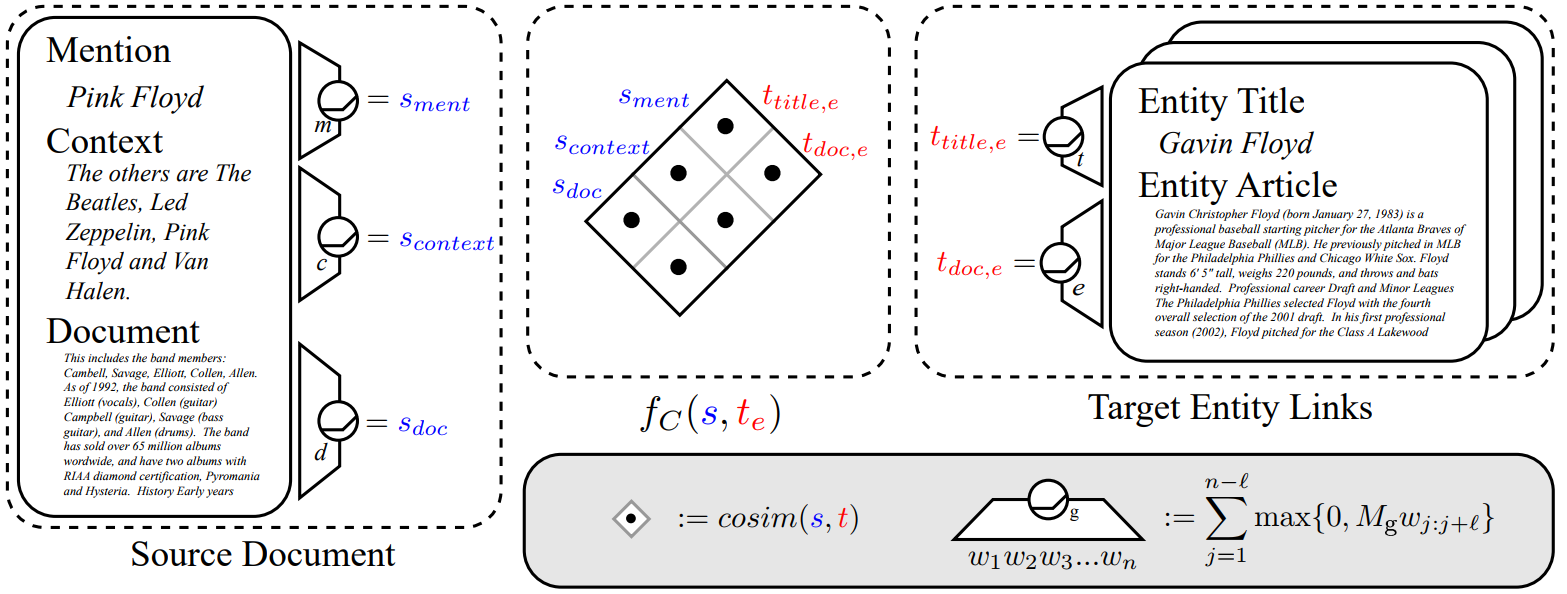
\includegraphics[width=0.95\columnwidth]{figure/rw/linking-francis.png}
	\bicaption{基于多粒度卷积神经网络的实体链接模型。\cite{francis2016capturing}}
    {Entity linking model with CNN at multiple granularities.}
	\label{fig:rw-linking-francis}
\end{figure}


%(68)[Pic][IJCAI] Modeling Mention, Context and Entity with Neural Networks for Entity Disambiguation (TAC-KBP数据集)
Sun等人\cite{sun2015modeling}的模型对不同的上下文信息
采用了不一样的网络结构。
如\figref{fig:rw-linking-sun}所示,
对短语建模的信息包括短语自身,以及去除自身后的句子两部分,
而实体方面,除了利用本身名称之外,还使用了它在维基百科中的分类信息,
用这类人工提炼的知识补充实体的表示。
对句子的表示学习依然使用卷积神经网络,
其余三种信息由于长度较短,均直接使用了词向量平均的方式得到向量表达。
进一步,该模型利用较为复杂的神经张量层将各部分向量结合,
分别得到实体和短语的整体表达。
%以捕捉向量不同维度间的信息交互。
类似的方法还有文献\parencite{gupta2017entity},
对实体的维基分类信息进行表示学习,
通过双向循环神经网络对短语所在句子进行编码。
同时模型定义了不同信息之间的多种损失函数,对训练数据的利用更加充分。
%(7)[Pic][EMNLP] Entity Linking via Joint Encoding of Types, Descriptions, and Context
%(6)[BadPic][COLING] Joint learning of local and global features for entity linking via neural networks (ref充数用,需要再加)

\begin{figure}[th]
	\centering
    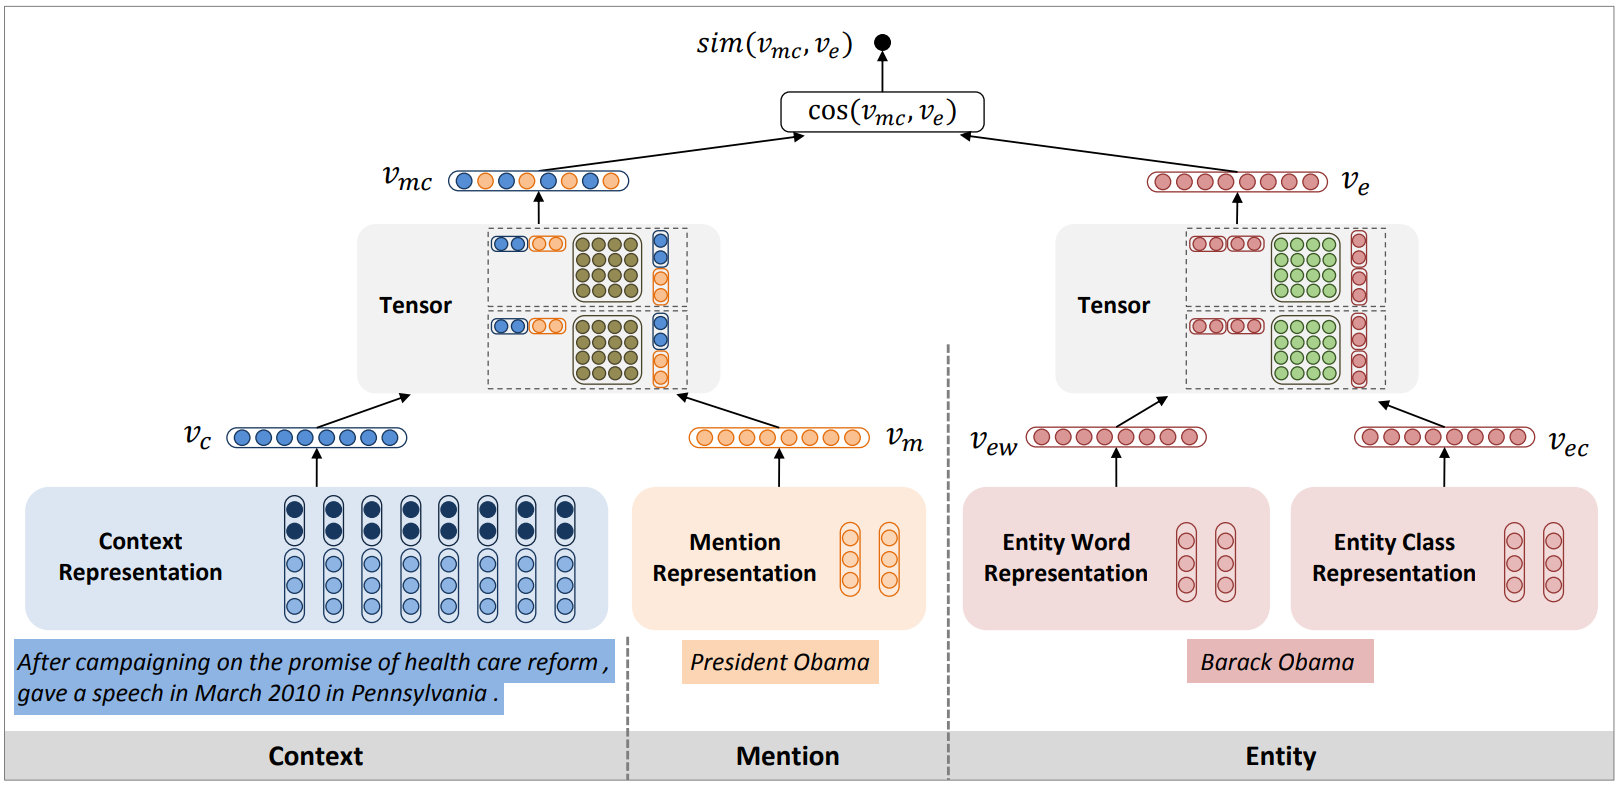
\includegraphics[width=0.95\columnwidth]{figure/rw/linking-sun.png}
	\bicaption{基于神经张量层的链接模型。\cite{sun2015modeling}}{NTN based entity linking model proposed by Sun et al.}
	\label{fig:rw-linking-sun}
\end{figure}

%(22)[NoPic][CoNLL] Entity Disambiguation by Knowledge and Text Jointly Embedding
此外,知识库向量学习技术\cite{bordes2013translating}也被用于实体链接任务中。
知识库向量学习与词向量学习类似,以大量事实三元组作为训练数据,
学习每个实体的向量表示,使得相近语义的实体具有相近的向量。
Fang等人\cite{fang2016entity}提出的链接模型基于知识库向量与词向量的融合:
通过实体与短语互相替代的方式,定义了基于三元组以及共现词对的目标函数,
促使实体与其短语的向量尽可能一致,因此所有向量表示被映射到同一个高维语义空间中。
融合的优势在于实体和单词之间直接可比,
通过距离度量函数计算候选实体与短语上下文中不同词的距离,
并以此作为链接模型的特征。

%(41)[NoPic][CoNLL] Joint Learning of the Embedding of Words and Entities for Named Entity Disambiguation(凑人头)
%(9)[Pic][EMNLP] Deep Joint Entity Disambiguation with Local Neural Attention(凑人头)


%"通过xxx得到xxx,因此可以对xxxx进行建模  进一步xxxx"



%出现在Tutorial里的
%Local and Global Algorithms for Disambiguation to Wikipedia (Ratinov)(Illinois Wikifier)
%Robust Disambiguation of Named Entities in Text (放图)(AIDA数据集)
%Linden: linking named entities with knowledge base via semantic knowledge
%Joint Named Entity Recognition and Disambiguation(EMNLP2015,CRF)(AIDA)
%S-MART(啥数据?)(啥特征?)
%不同特征对应的不同类型。



%\subsection{跨语言场景的实体链接模型}
%\label{sec:rw-linking-bilingual}


\subsection{跨语言词向量}
\label{sec:rw-linking-cle}

上一节的论述中提到了词向量模型,用于学习词汇的连续语义表示,但仅局限于单一语言。
对于涉及多个语言的任务,难点在于如何实现语义的跨语言过渡。
为了解决此问题,跨语言词向量模型(Cross-Lingual Embedding Model)
旨在消除单词语义表示对语言的依赖,
将不同语言的向量表示映射至同一连续空间,并依旧保持相似语义单词更加接近的特性,
以此实现语义迁移。
例如\figref{fig:rw-linking-cle}展示了一个英语和德语之间的共享语义空间,
可以清晰地识别出两种语言间的许多组翻译词对。

\begin{figure}[th]
	\centering
    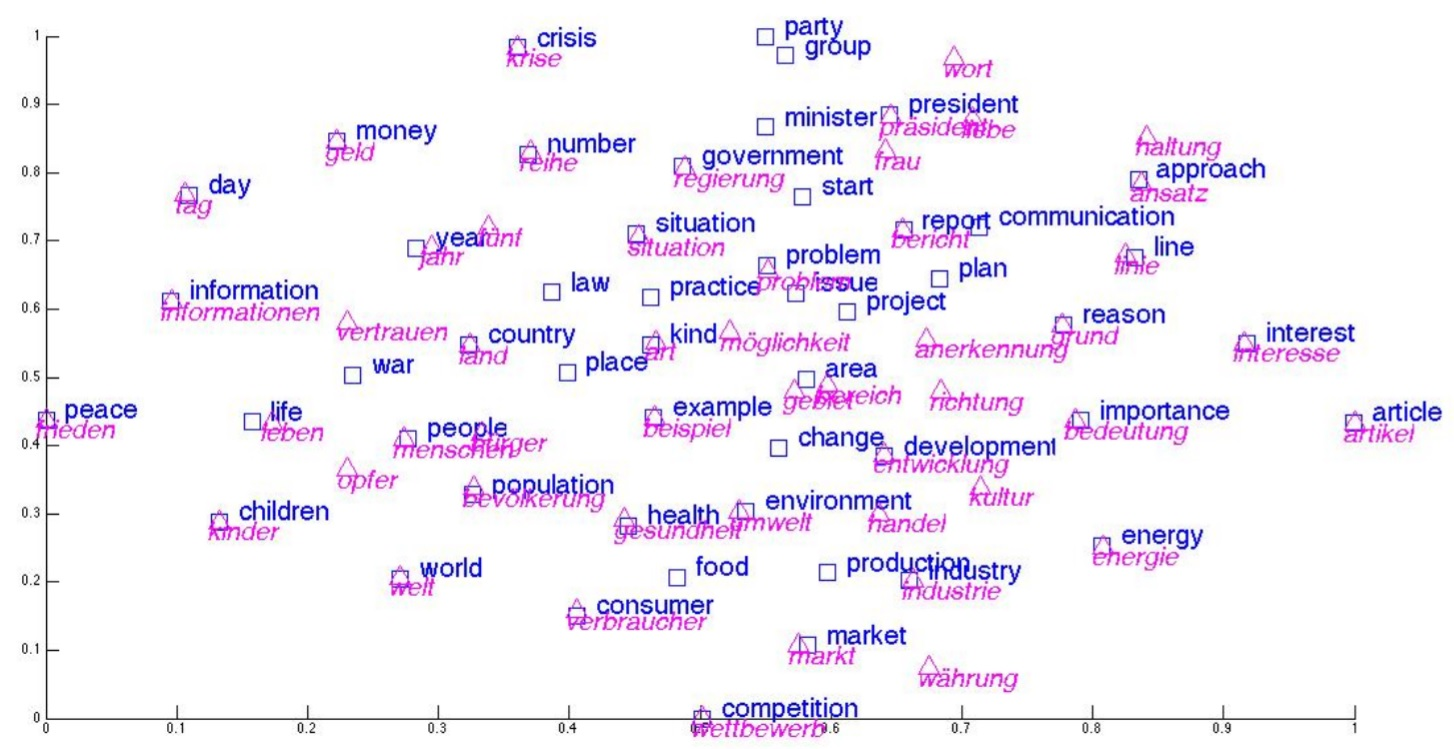
\includegraphics[width=0.8\columnwidth]{figure/rw/linking-cle.jpg}
	\bicaption{英语和德语间的跨语言词向量例子。\cite{ruder2017survey}}
    {An example of cross-lingual word embeddings between English and German.}
	\label{fig:rw-linking-cle}
\end{figure}

跨语言词向量的训练,需要依赖平行语料库用于给模型提供语义对齐信号,
不同的训练方式区别在于平行语料的类型不同,
例如单词级别\cite{mikolov2013exploiting,klementiev2012inducing,lazaridou2015hubness}、
句子级别\cite{hermann2013multilingual,gouws2015bilbowa}、
文档级别\cite{vulic2016bilingual}的对齐。
利用单词级别对齐进行跨语言词向量训练的工作最为普遍,
训练数据主要来自于双语或多语词典中抽取出的高质量翻译词对。
以此为例,对于源语言$s$和目标语言$t$,模型的损失函数$J$由三部分组成:
\begin{equation}
  J = \mathcal{L}_{mono}^{s} + \mathcal{L}_{mono}^{t} + \Omega{}^{s \rightarrow t},
\end{equation}
\noindent
其中,$\mathcal{L}_{mono}$代表各自语言上进行单语言词向量训练的损失,
可直接使用CBOW等已有模型进行计算,
而$\Omega{}^{s \rightarrow t}$为正则项,对应单词对齐的损失。


对于$\Omega{}^{s \rightarrow t}$的定义,相关文献进行了不同的尝试。
Mikolov等人\cite{mikolov2013exploiting}发现,
在不同语言中,多个单词的向量表达之间,几何关系较为相似,
例如英语和西班牙语中,表示数字的单词之间的相对位置几乎一致,
表示动物的单词也有类似特性。
基于以上观察,该工作提出的模型使用了线性变换的方案,
训练转移矩阵$\bm{W}$(或称投影矩阵),
使得源语言词向量$\bm{x}^{s}$经过$\bm{W}$投影后,和对齐的目标语言词向量$\bm{x}^{t}$
的欧氏距离平方(即均方误差)尽可能小:
\begin{equation}
  \Omega{}^{s \rightarrow t} = \sum_i { \| \bm{Wx}_i^s - \bm{x}_{i}^{t}  \|^{2} },
\end{equation}
\noindent
基于线性映射的跨语言词向量模型具有一些变种,
例如文献\parencite{xing2015normalized,zhang2016ten}限制转移矩阵$\bm{W}$为单位正交阵,
以保证映射后的词向量维持单位长度,
Artetxe等人\cite{artetxe2016learning}指出,对于模型效果而言,
转移矩阵正交化比向量正则化更加重要。
Lazaridou等人\cite{lazaridou2015hubness}对$\Omega{}^{s \rightarrow t}$的定义使用了最大间隔(Max Margin)损失
来代替均方误差损失,即不追求$\bm{Wx}^s$与$\bm{x}^t$绝对距离尽可能小,
而是让$\bm{x}^t$比其它任何不相关单词都更加接近$\bm{Wx}^s$,
从而避免跨语言词向量出现过多中枢词的现象。
Faruqui等人\cite{faruqui2014improving}利用
典型相关分析(Canonical Correlation Analysis, CCA)\cite{hotelling1936relations}
进行词向量训练。CCA同为线性投影方式,不同之处在于,
%也可用于将不同语言的词向量线性投影到同一个向量空间中,与之前的线性映射不同,
CCA对两个语言分别学习一个线性变换矩阵,
目标是尽可能降低映射后每个翻译词对的互协方差分值。

%训练过程:分开,joint
%(稍微扯一下优点,虽然还没想好)
此外,跨语言词向量的训练还可
对于通过句子或文档级别的平行语料进行跨语言词向量的训练,由于不是本文的研究重点,
故不展开论述。
跨语言词向量能够应用在多种任务中,
例如文档分类\cite{klementiev2012inducing}、词性标注\cite{zhang2016ten}、
命名实体识别\cite{murthy2016sharing}、机器翻译\cite{zou2013bilingual}等,
其带来的知识迁移具有很高的实用性。
对于训练集和测试集为不同语言的任务,跨语言词向量能实现知识在不同语言上的迁移;
对于类似机器翻译、跨语言实体链接等输入和输出为不同语言的任务,
预训练好的跨语言词向量能够作为特定任务模型的训练起点,
消除语义的间隔,从而提升整体效果。


%Zhang IJCAI 2012 Cross Lingual Entity Linking with Bilingual Topic Model

%Sil AAAI 2018 Neural Cross-Lingual Entity Linking (先放着,来不及了)
%Tsai NAACL 2016 Cross-lingual Wikification Using Multilingual Embeddings (留给小RW)


%Entity linking or wikification is another task tackled using cross-lingual word embeddings
%(Tsai & Roth, 2016). The purpose of the task is to ground mentions written in nonEnglish
%documents to entries in the English Wikipedia, facilitating the exploration and
%understanding of foreign texts without full-fledged translation systems (Ji, Nothman,
%Hachey, & Florian, 2015). Such wikifiers, i.e., entity linkers are a valuable component
%of several NLP and IR tasks across different domains (Mihalcea & Csomai, 2007; Cheng
%& Roth, 2013).







%# -*- coding: utf-8-unix -*-
% !TEX program = xelatex
% !TEX root = ../thesis.tex
% !TEX encoding = UTF-8 Unicode

\section{关系理解:知识库补全任务}
\label{sec:rw-kbc}

%Part 1: 什么是KBC

现有的知识库具包含了庞大数量的实体和事实,但其中的内容仍然不够完全,
尤其是存在大量的长尾实体,并没有多少事实与之相关。
因此,知识库补全任务(Knowledge Base Completion, KBC)的目的,
是向已有知识库中添加缺失的事实三元组($e_1$, $p$, $e_2$)。
这些新增的三元组中,无论是谓词$p$还是它的两个参数实体$e_1$和$e_2$,
都已存在于知识库中。
换言之,新增的事实并不会给知识库带来额外的节点,或是从没见过的边,
而是让知识库的图结构更加稠密。

新增事实三元组(尤其是参数实体)的获取方式通常有两种。
第一种来源为经过了实体链接过后的外部文本,纯文本或表格文本均可称为来源。
%
对于纯文本,当在句中定位两个参数实体后,
句子剩下的部分成为了描述实体间关系的上下文。
此时即可依据上下文信息来预测对应的知识库谓词,
即等价于关系分类问题,相关研究包括词级别卷积神经网络\cite{xu2015semantic}
以及依存语法路径上循环神经网络\cite{xu2015classifying}。
对于表格文本,知识库补全关注于表格的两列之间,利用表列所包含的实体,
判断两列之间的关系是否与知识库中特定谓词对应,实现可能的大批量事实补全。
例如\figref{fig:rw-linking-limaye},
Title和Author列之间的关系被映射到YAGO中的$Writes$谓词。
%主要使用的方法有
%如概述中指出,  表格关系可以补充三元组
%Munoz:找关系 挖掘不同行之间,但是是同样的两列之间的实体关系,映射至DBPedia 构成三元组,即挖掘语义。  并补充缺失
%在维基百科内部(已有链接)
%按已有match比例尝试一些predicate,然后学习一个triple是对还是错
%Sekhavat: Tabular KBC 同样是假设linking已好的情况 利用PATTY作为跳板,根据EP之间存在的pattern,寻找到rel的关系
%条件概率  (相当于EP有一系列的外部文本pattern,而不是仅有KB)
%rel来自YAGO
%(Fuck...但两者根本都是column-column-rel和predicate的一一对应)

第二种来源不涉及到任何知识库外的信息,新增三元组来自于知识库的内部挖掘,
通过寻找不同谓词之间的关联,推理出可能缺失的事实。
例如\secref{sec:intro-background}提到的例子,
``{某人的国籍缺失,可以根据其出生地所在的国家进行推测}'' ,
人类可以通过这样的方式进行知识的手动补充,正是因为掌握了
国籍、出生地、地点被包含这三个谓词之间的关联。
这条路线不受知识库外信息的干扰,因此是我们关注的研究点。

学术界已有工作在此场景上研究知识库补全的解决方案,
并提出了相关的KBC数据集,
例如FB15k\cite{bordes2013translating}和WN18\cite{bordes2014semantic},
分别是Freebase和WordNet的子集。
对于知识库补全模型的测评,主要通过
主宾语预测(Link Prediction)以及三元组分类(Triple Classification)
这两个子任务来进行。
前者为三元组($e_1$, $p$, $?$)或($?$, $p$, $e_2$)预测缺失的主语或宾语,
后者则判断给定的($e_1$, $p$, $e_2$)是否为正确事实。
两者虽然形式不同,但都需要计算三元组的置信分:$S(e_1, p, e_2; KB)$。

解决知识库补全的方法主要分为两类。
第一类基于规则推导,用逻辑表达式描述实体间存在特定谓词时,所需要满足的特定规则;
第二类基于知识库向量,学习所有实体、谓词的连续特征表示,
并挖掘三元组各部分特征表示之间存在的深层代数关系。
下面将分别介绍这两种方法。

\subsection{基于规则推导的模型} %基于规则推导的关系语义推理模型

基于规则推导的模型旨在使用人类可以直接理解的规则形式,来描述不同谓词之间的联系,
即如果$e_1$和$e_2$之间满足特定的条件,则推理出三元组($e_1$, $p$, $e_2$)成立。
为方便论述,我们将三元组以布尔表达式$p(e_1, e_2)$表示,
若对应三元组存在于知识库中,则表达式为真,否则表达式为假。
文献\parencite{lao2011random}以一个简单的推导规则为例:
若已知某运动员为球队效力,以及球队所处联盟,则可以推导出运动员所参与的体育联盟。
该规则可以通过一阶逻辑表达式进行形式化描述:
\begin{equation}
\begin{aligned}
\exists b \in E, athletePlaysForTeam(a, b) & \land teamPlaysInLeague(b, c) \\
                                           & \implies athletePlaysInLeague(a, c),
\end{aligned}
\end{equation}
\noindent
其中$E$表示知识库实体集合。规则的左侧部分,使用的两个谓词实现了主语$a$到宾语$c$的连接,
且不包含多余的布尔表达式,因此这条规则表现为由谓词序列构成的路径。
对于``{依靠出生地推测国籍}'' 的规则,我们可以形式化为以下逻辑表达式:
\begin{equation}
\begin{aligned}
  \exists b \in E, placeOfBirth(a, b) & \land containedBy(b, c) \\
                                      & \land isA(c, country) \implies nationality(a, c),
\end{aligned}
\end{equation}
\noindent
其中谓词序列$\{placeOfBirth, containedBy\}$为连接主宾语的路径,
而谓词$isA$使得宾语$c$还需要满足额外的限制条件,因此这条规则具有比路径更加复杂的结构。

利用单个推导规则进行知识库补全存在两个局限:
首先,规则本身不一定完全正确,限制条件过于宽泛的规则可能打来错误的事实;
其次,单个规则的覆盖率较低,能够补全的知识有限。
针对这两个局限,已有的规则推导工作都致力于从知识库中挖掘目标谓词的多条规则,
并学习不同规则的重要性,以实现更健壮的知识库补全。

Lao等人提出的PRA模型\cite{lao2010fast}实现了规则的挖掘和学习。
对于目标谓词$p$,模型首先利用谓词已有的三元组($e_1$, $p$, $e_2$)作为训练数据,
在知识库中寻找所有能连通$e_1$和$e_2$的谓词序列,形成了多种路径形式规则。
模型利用逻辑回归实现规则权重的训练,以及对新三元组($e'_1$, $p$, $e'_2$)是否为真的预测。
每一条挖掘的规则类比为一个特征,对应的特征值为路径随机游走概率,
即从主语$e'_1$出发,沿规则的谓词序列随意跳转,最后到达$e'_2$的概率。
由于知识库中的谓词可能代表一对多关系,
因此随机游走概率值会小于1,甚至为0(无法通过当前规则连通)。
基于此,PRA模型能够快速抽取大量路径规则,并利用已知三元组在规则上随机游走概率实现权重训练。

一些研究工作对PRA模型进行了扩展。
文献\parencite{lao2011random}对挖掘的路径规则进行了限制,
要求规则至少要适用于训练数据中一定比例的主语,并对计算随机游走概率的采样方式进行了优化,
这两个扩展都是基于模型性能优化为考量。
%lao2011random
%改进1: 限制每条路径规则所能  满足的主语个数  以及连通的 训练三元组个数,  大幅度缩小规则数量
%改进2:随机游走的采样方式进行了优化。
Gardner等人提出了SFE模型\cite{gardner2015efficient},它在PRA模型基础上进行了两项改进:
首先,模型将作为特征值的随机游走概率替换为0/1特征,即只关心是否连通,
在大幅度提升运行速度的同时,对结果没有显著影响;
其次,模型引入不同于路径规则的其它特征,例如提取路径中的谓词bigram,
或由主语出发却不指向宾语的单边特征等,扩充特征集合以提升知识库补全效果。
%gardner2015efficient
%改进1:特征值转换为0/1对结果没有显著影响,PRA的具体概率值并不比0/1提供了更多信息(很惊讶),而PRA概率计算花费了大量时间
%改进2:引入了更多的规则,单边  anyrel, path bigram   并非基于路径的规则 but useful
Wang等人提出了CPRA模型\cite{wang2016knowledge},主要针对具有相似谓词的规则推导优化。
该模型通过层次聚类识别出具有相似语义的知识库谓词集合,
然后对每个集合内的谓词采用多任务学习框架,共享挖掘的规则特征和部分耦合参数,
使模型能够捕捉相似谓词之间的共性,实现隐式的训练数据共享。
%wang2016knowledge
%针对具有相似语义的知识库谓词,对它们的关系推理 过程   不独立,而是 能 彼此利用训练数据  互相影响,
%提出了  CPRA模型,   通过层次cluster识别  相似语义 的知识库谓词 ,   多任务学习 等方式 学习,
%使得  不同谓词的规则推导 不完全独立,   可以利用其它 的训练数据  优化自身。

%TODO: AMIE+, Zhang的放在内部related work说,有点太细了
% AMIE+
% 
% Zhang等人的研究 是 此任务 较早的工作。
% 文中称Ontological Smoothing, 为 特定关系寻找更多seed pair,
% 并用于relation extraction中,以提高pattern的准确率。
% 虽并不称作kbc,但本质相同。
% 提出了基于MLN的模型。
% 不仅
% 对每个谓词生成的规则由长度不超过4的谓词序列
% 同时对NELL 中的e和t都映射
% 
% 使用MLN学习每个规则的权重
% 对每个 谓词 相关规则   都寻找  合适的表达式,   谓词序列  考虑 并集
% 
% (类似的文章还有SQL query generation,见他的RW)
% 
% Zhang,MLN。。。
% %说各自的弱点
%   title={Learning to refine an automatically extracted knowledge base using markov logic},
%     goal: 过滤NELL,在candidate facts里寻找正确的fact。
%     rules: 好像并没有直接去学习p和p之间的关联,而是和meta predicate在搞?
%     model: MLN
%     
%   title={Large-scale knowledge graph identification using psl},
%     goal: 同上
%     rules: extractor, ontological, isA, relation
%     model: PSL, weight on rule, and also on the atom expression (KALE)
% 
%   title={Statistical schema induction},
%     太长了,先忽略
% 
% 
% 然后就终结在这里。不要再多了,ball ball u.

\subsection{基于知识库向量的模型}

与词向量模型类似,知识库向量的模型旨在学习一个知识库中的实体、谓词等元素
在连续空间的特征表达,以完成一系列下游任务。
具体在知识库补全任务中,
三元组置信分的计算并不依赖自动挖掘的推导规则,
而是来自主谓宾三者的连续特征表达在不同维度上的交互。
词向量模型依靠大规模的纯文本语料,
构建上下文单词预测任务来完成训练\cite{mikolov2013exploiting},
相比之下,知识库向量模型的训练过程更为直观:
利用知识库已有三元组作为训练数据正样本,
并自动生成不存在的三元组作为负样本,计算三元组置信分进行训练,
而这也恰好与知识库补全任务的目标一致。

知识库向量模型的优点在于所有谓词共同训练,更有效地利用训练数据,
并且能在连续空间中体现不同谓词的相似性,
但相应地,其缺点在于可解释性较弱。
不同的知识库向量模型对实体和谓词的特征表示具有不同的形式,
特征交互的方式也不尽相同,下面主要介绍几个具有代表性的模型。
%一类以RESCAL为代表,多层网络输出multi-layer perc;一类以TransE为代表,latent distance model

%类比词向量的训练,CBOW 等 依据上下文进行预测,相似语义 相似上下文
%类似的思路,信息来自已有的事实三元组,相似的实体 会有相似的谓词和另一个实体
%对于谓词也有类似的性质
%然而,上下文信息由三元组表示,准备好了更加准确的训练数据。
%以及实体和谓词并不是同一类东西,不能像word2vec那样,实体和谓词会在不同的空间中。
%From: A review of relational machine learning for knowledge graphs


\begin{figure}[htp]
  \centering
  \subcaptionbox{RESCAL模型\label{fig:rw-kbe:a}}
    {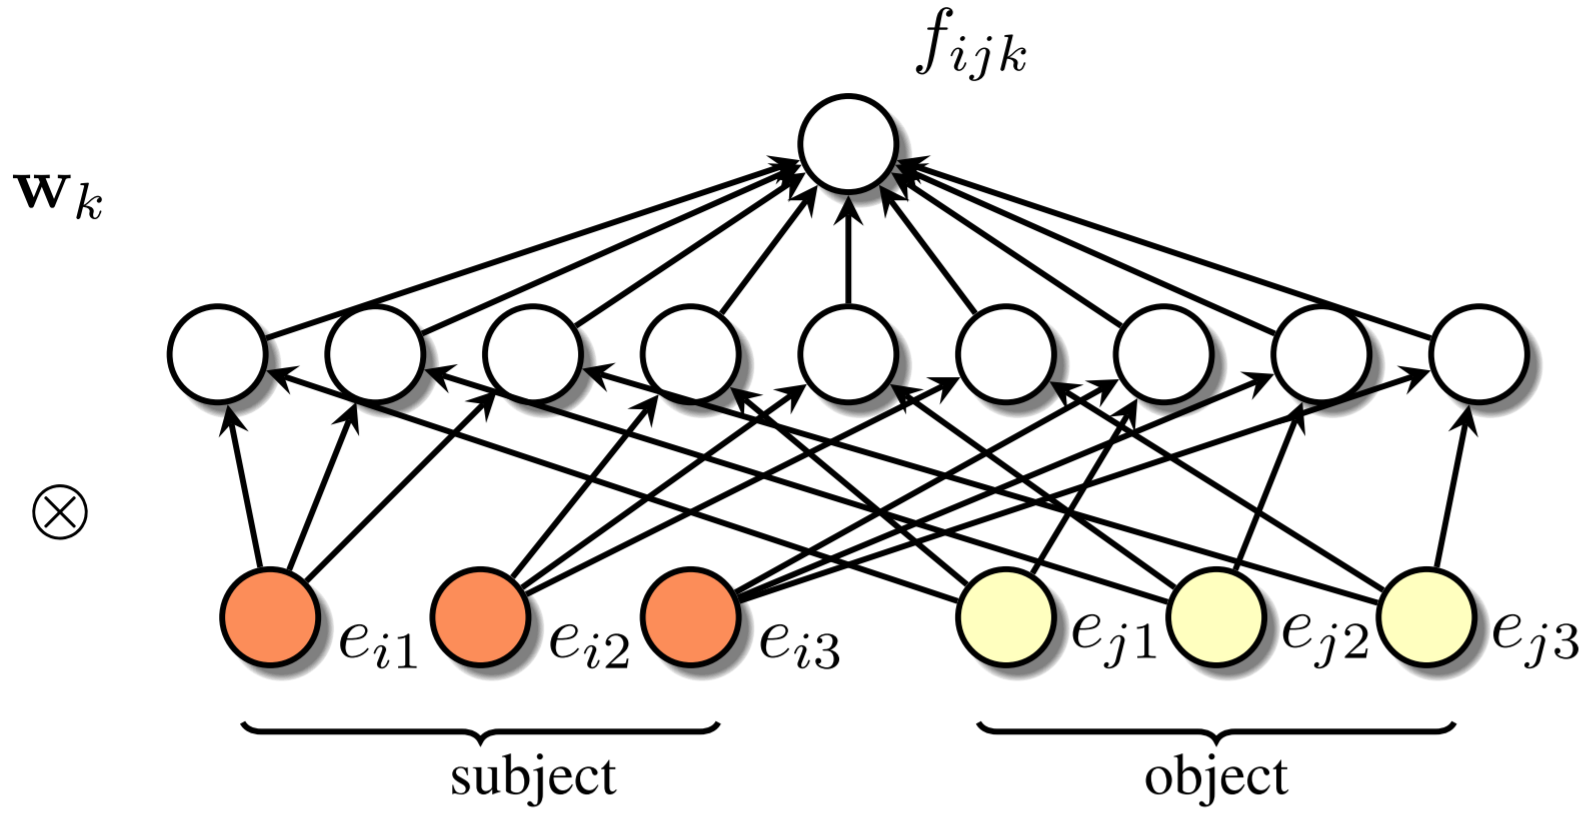
\includegraphics[width=0.48\columnwidth]{figure/rw/kbc-rescal.png}}
  \hspace{1em}
  \subcaptionbox{ER-MLP模型\label{fig:rw-kbe:b}}
    {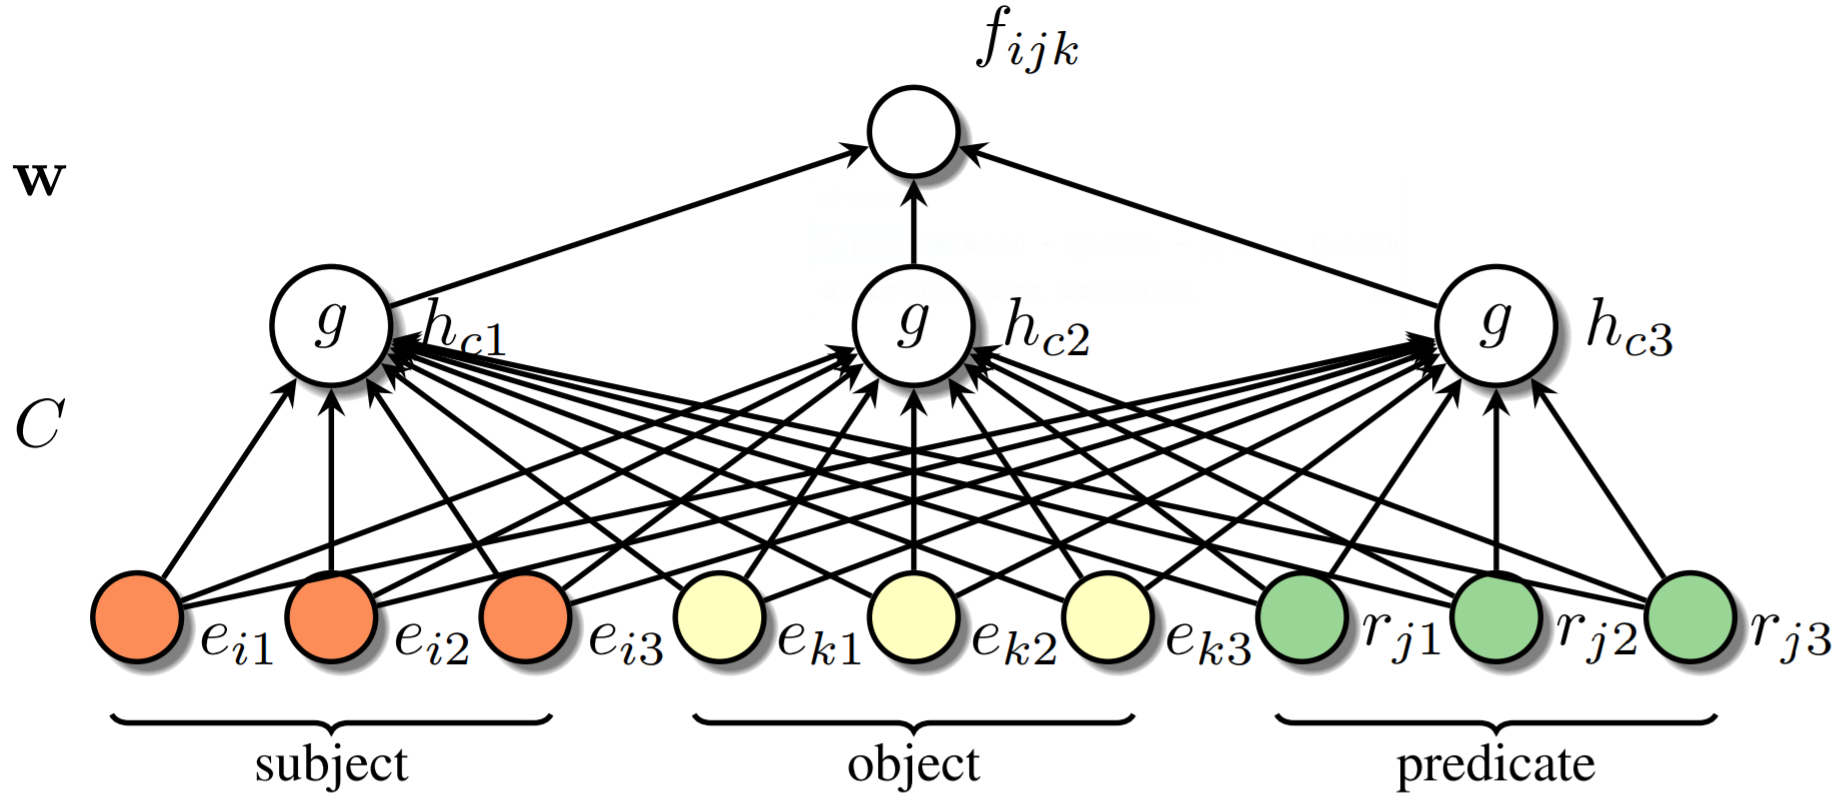
\includegraphics[width=0.48\columnwidth]{figure/rw/kbc-ermlp.png}}

  \vspace{1em}

  \subcaptionbox{TransE模型\label{fig:rw-kbe:c}}
    {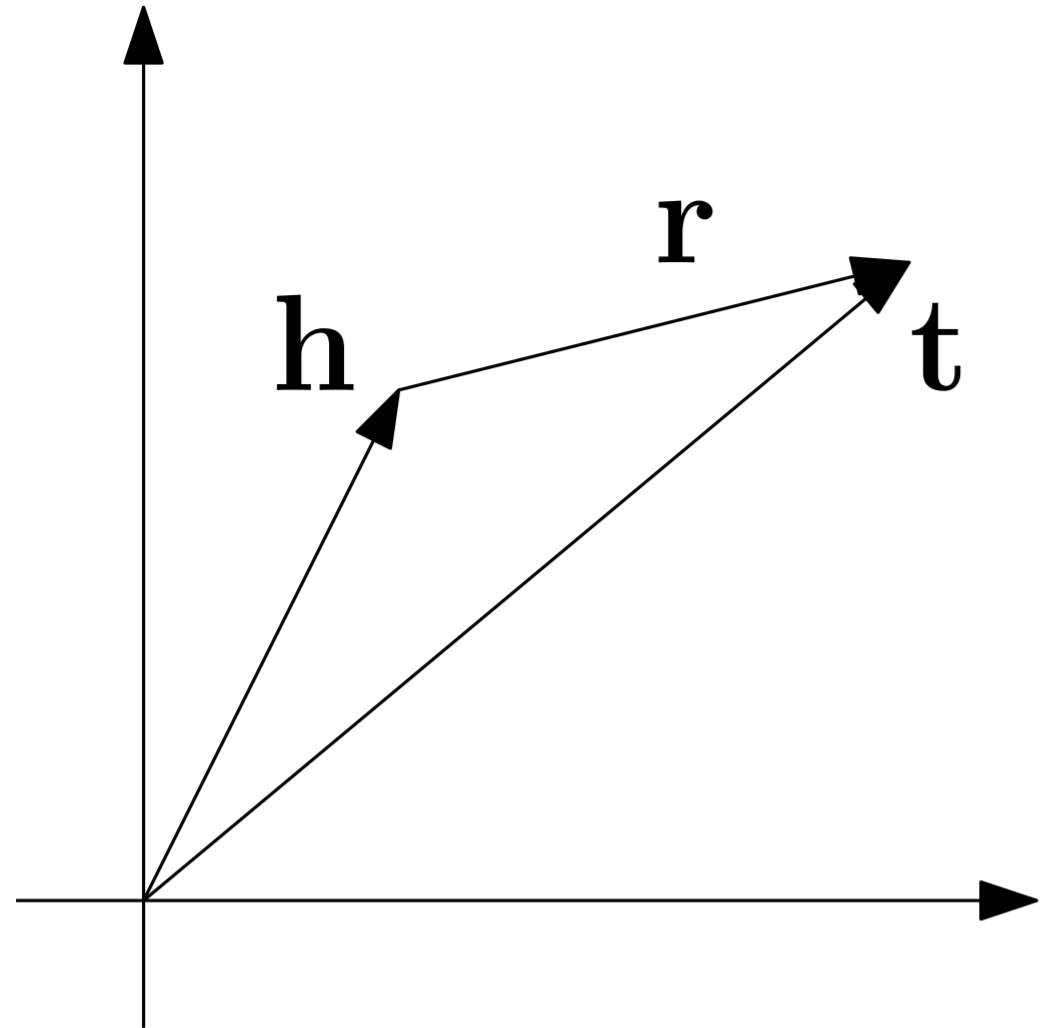
\includegraphics[width=0.30\columnwidth]{figure/rw/kbc-transe.png}}
  \hspace{4em}
  \subcaptionbox{TransH模型\label{fig:rw-kbe:d}}
    {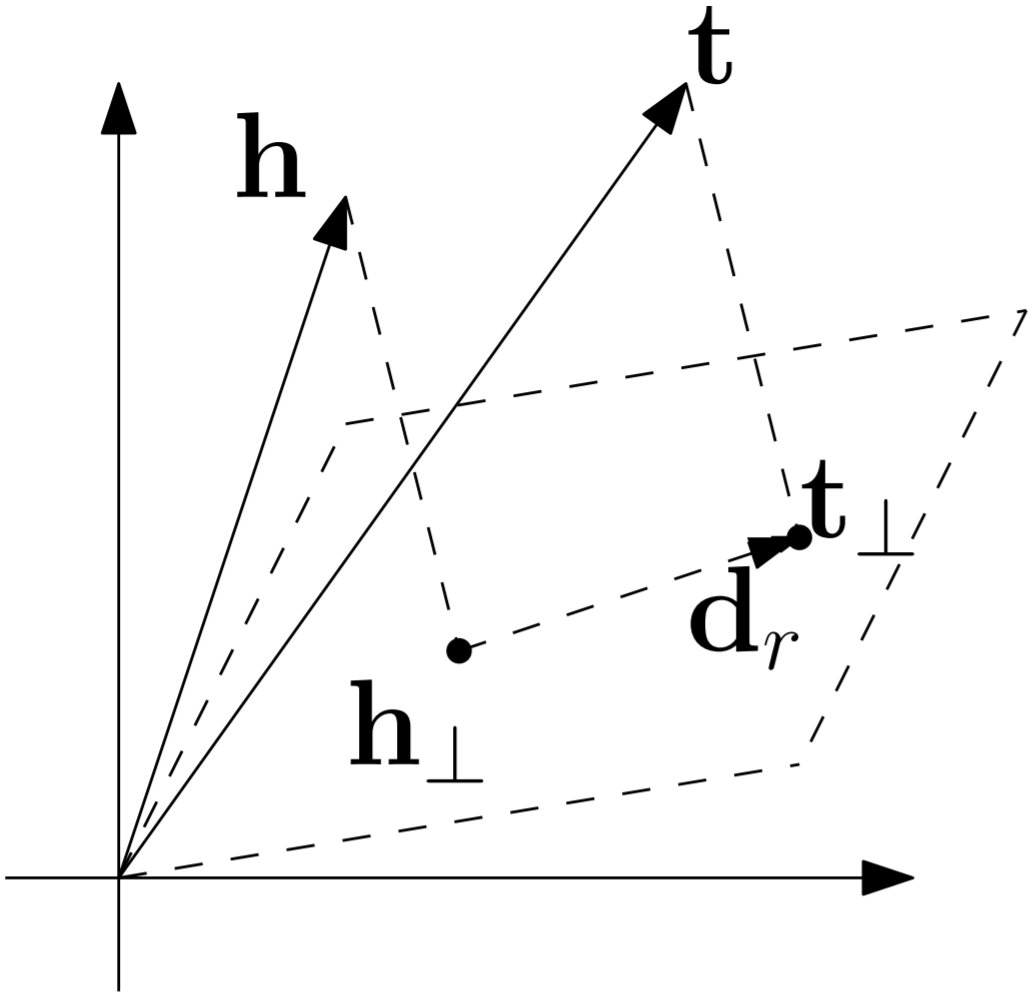
\includegraphics[width=0.30\columnwidth]{figure/rw/kbc-transh.png}}
  \bicaption{多种知识库向量模型示意图。\cite{nickel2016review,wang2014knowledge}}
            {Examples of knowledge base embedding models.}
  \label{fig:rw-kbe}
\end{figure}


由Nickel等人提出的RESCAL模型\cite{nickel2012factorizing}是一个基础的知识库向量模型,
模型对三元组($e_i$, $r_k$, $e_j$)置信分(简写为$S$)的定义,
基于主宾语实体特征表示的在不同维度间的两两交互:
\begin{equation}
S^{RESCAL} = \bm{e}_i^\top \bm{W}_k \bm{e}_j = \sum_{a=1}^d \sum_{b=1}^d w_{kab} e_{ia} e_{jb},
\end{equation}
\noindent
其中$\bm{e}_i$和$\bm{e}_j$为对应实体向量,维度为$d$。$\bm{W}_k \in \mathbb{R}^{d \times d}$
为谓词$r_k$的权重矩阵,其中$w_{kab}$体现了实体向量的第$i$和$j$维特征对于第$k$个谓词的交互重要性。
由于RESCAL使用矩阵连乘形式捕捉实体向量之间的交互,因此也被称为双线性模型。
如\figref{fig:rw-kbe:a}所示,RESCAL模型可表示为双层神经网络结构,
首先通过张量积(Tensor Product)构建实体对($e_i$, $e_j$)的组合特征,
再利用与特定谓词相关的参数$\bm{W}_k$作为权重,得到三元组最终的置信分。
RESCAL模型学习的实体特征表示能够捕捉不同实体间的语义相似性,
换言之,若两个实体可以通过相似的谓词连接至相似的其它实体,
那么它们的特征表达也更加相近。

%The shared entity representations
%in RESCAL capture also the similarity of entities in the
%relational domain, i.e., that entities are similar if they are
%connected to similar entities via similar relations [65].


RESCAL模型存在的一个问题在于参数量过大,每一个谓词对应参数量为$d \times d$,
对于拥有大量谓词的知识库而言,会带来可扩展性的问题。
一些后续研究对此进行了改进。
Socher等人以及Dong等人
分别提出了E-MLP\cite{socher2013reasoning}和ER-MLP模型\cite{dong2014knowledge}。
\figref{fig:rw-kbe:b}为ER-MLP的示意图,均由两层前向网络构成,
第一层用于学习三元组的组合特征表示,第二层则通过组合特征输出置信分。
E-MLP结构较为类似,故此处不专门画图。
两个模型的置信分计算如下:
\begin{equation}
\begin{aligned}
& S^{E-MLP} = \bm{w}_k^\top \bm{g}(\bm{C}_k [\bm{e}_i; \bm{e}_j]), \\
& S^{ER-MLP} = \bm{w}^\top \bm{g}(\bm{C} [\bm{e}_i; \bm{e}_j; \bm{r}_k]),
\end{aligned}
\end{equation}
\noindent
其中,$g$为非线性激活函数。
对比RESCAL模型,E-MLP的最大不同在于可以通过调整矩阵$\bm{C}_k$来学习实体间不同维度特征的交互,
从而优化实体对($e_i$, $e_j$)的组合特征表示,并大幅度减少参数数量。
E-MLP模型中,不同的谓词依然对应不同的参数,而ER-MLP模型将谓词也映射为向量表示,
与两实体共同作为第一层的输入,因此模型的参数$\bm{C}$与$\bm{w}$均与特定谓词无关。
两个模型依然能够让语义相似的实体映射至连续空间的相近位置。

Nickel等人提出了HOLE模型\cite{nickel2015holographic},
该模型利用循环相关运算(Circular Correlation)巧妙地代替了RESCAL中的张量积操作:
\begin{equation}
S^{HOLE} = \bm{w}_k^\top (\bm{e}_i \star \bm{e}_j) = \sum_{a=1}^d \sum_{b=0}^{d-1} w_{ka} e_{ia} e_{j,(a+b) \% d},
\end{equation}
\noindent
可以从公式中看出,循环相关运算等同于将张量积的结果进行了分组,模型通过对实体特征表示的学习,
让具有相似语义的特征交互归为同一组,共享同一个权重。
因此HOLE的优势在于将RESCAL中的二维矩阵参数降低至一维,同时尽可能保留了特征交互的表示能力,
并且在实验中效果优于RESCAL和ER-MLP模型。

此外,Socher等人还提出了较复杂的神经张量网络(Neural Tensor Networks,NTN)模型\cite{socher2013reasoning},
可以看做是RESCAL和E-MLP的组合体,对实体对($e_i$, $e_j$)构建的组合特征表达同时包括双线性和前向网络特征,
但模型参数量也因此更加庞大,在小数据集上更容易出现过拟合。



%1+3+1段
另一类 知识库向量模型   是以TransE为典型的 被称作 隐距离模型。
相比 RESCAL等模型 依照神经网络构建的置信分函数,
隐距离模型对置信分的计算则与距离度量直接相关。
这与\secref{sec:rw-linking-cle}介绍的跨语言词向量训练有着相似之处,
源语言词向量经过转换后,与翻译后的词向量尽可能相近。
而对于知识库向量模型,由于三元组中还有谓词的存在,
因此模型训练的实质,是学习主宾语实体向量在特定谓词下的变换方式,
对变换之后的向量表示进行距离度量,距离越近,则置信分越高。
为了和相关工作统一,此处用($h$, $r$, $t$)表示一个事实三元组。

Bordes等人提出的SE模型\cite{bordes2011learning}较为基本,
度量实体$h$和$t$经矩阵变换后的距离:
\begin{equation}
S^{SE} = -dist(\bm{A}_r^s \bm{h}, \bm{A}_r^o \bm{t}),
\end{equation}
\noindent
其中$dist(\cdot)$为距离度量函数,例如L1距离或欧氏距离。
谓词$r$对应两个参数矩阵,分别映射主语和宾语实体的向量表示至同一空间。
为了降低参数个数,Bordes等人提出了TransE模型\cite{bordes2013translating},
这也是后续很多改进模型的起点。
受到词向量之间代数运算的启发,
例如$queen \simeq king - man + woman$\cite{mikolov2013linguistic},
不同词之间的关系体现在了它们词向量的位置偏移中,
因此如\figref{fig:rw-kbe:c}所示,TransE模型共享了实体与谓词的特征表示,
利用在主语实体在同一空间中的平移变换,代替更加复杂的矩阵变换:
\begin{equation}
S^{TransE} = -dist(\bm{h} + \bm{r}, \bm{t} ).
\end{equation}

TransE模型设计简单、容易实现,并且具有训练速度快、可扩展性高等优点,
但是对于知识库中存在的一对多或多对一的谓词不友好,
例如固定主谓,TransE无法有效区分出多个匹配的宾语实体。
为此,TransH模型\cite{wang2014knowledge}尝试通过超平面投影来解决此问题,
公式定义如下:
\begin{equation}
  \bm{h}_\bot = \bm{h} - \bm{w}_r^\top \bm{h} \bm{w}_r, \ 
  \bm{t}_\bot = \bm{t} - \bm{w}_r^\top \bm{t} \bm{w}_r, \
  S^{TransH} = -dist(\bm{h}_\bot + \bm{d}_r, \bm{t}_\bot),
\end{equation}
\noindent
如\figref{fig:rw-kbe:d}所示,TransH首先把$h$和$t$的向量表示均投影到连续空间中,
谓词$r$对应的超平面上($\bm{w}_r$为单位法向量),
并学习谓词向量表示$\bm{d}_r$,在超平面上沿用TransE的度量。
因此,TransH具有更高的灵活度来应对一对多或多对一谓词,
同时依然保有TransE可扩展性高的特点。
TransR模型\cite{lin2015learning}同样尝试解决一对多谓词的问题,
类似于SE和TransE的组合体,利用投影矩阵$\bm{M}_r$将实体表示转移至新的空间后,
再进行基于平移的距离度量。
因此TransR模型中,实体和谓词的特征表达并不共享同一个语义空间,
这与TransE和TransH模型均不同:
\begin{equation}
S^{TransR} = -dist(\bm{M}_r \bm{h} + \bm{r}, \bm{M}_r \bm{t}).
\end{equation}

此外,还有其它TransE模型的改进工作,
包括体现距离度量在不同特征维度间差异的TransA\cite{xiao2015transa},
生成谓词多个表示以解决一对多问题的TransG\cite{xiao2016transg}等,这里不再展开讨论。

   %关系语义推理,别叫知识库补全
%# -*- coding: utf-8-unix -*-
% !TEX program = xelatex
% !TEX root = ../thesis.tex
% !TEX encoding = UTF-8 Unicode

\section{问句理解:知识库自动问答任务}
\label{sec:rw-qa}


自动问答任务是一类以自然语言问句为输入,并自动给出对应答案的任务。
基于知识库的自动问答(Knowledge Base Question Answering, KBQA)
是其中的一个热门研究方向,也是本文重点关注的问题。
在此问答任务中,输入问句为来自开放领域的事实类问句(Factoid Question),
即问句本身描述的是与某些特定实体相关的客观事实,
对应的答案通常表示为知识库中的实体、时间、数值等简单形式,
因此类似 ``how'' ``why'' 等以完整句子作为答案,或事实涉及到主观判断的问题,
不在任务的考虑范围之内。
以一个简单的英文问句为例,问句 ``what state borders texas?''
描述了与德克萨斯州相关的事实,其答案有多个,
包括New Mexico,Oklahoma,Arkansas,以及Louisiana四个实体。

对于知识库问答任务,使用的外部信息显然为结构化知识库。
正确答案的获取依赖于问答模型对问句整体语义的理解:
一方面准确定位问句中出现的相关实体,并链接至知识库;
另一方面根据问句信息,推理出未知答案与相关实体在知识库中具有的关系。
前者涉及到实体链接技术,后者体现了问句与知识库的语义匹配,也是问答模型的核心。
为了衡量问答模型对不同类型问题的效果,
学术界已提出了大量知识库问答数据集,
例如对问句进行结构化语义标注的QALD\cite{cimiano2013multilingual}和Free917\cite{cai2013large},
以及具有更大规模问答数据量的WebQuestions\cite{berant2013semantic}
和SimpleQuestions\cite{bordes2015large}等。

%和检索式问答  相比, 知识库问答    两者最大的差别在于答案来源  外部信息  的不同。
%对于检索式问答   以Squad为例
%对比检索式问答,   答案来自于给定的  文本,  抽取出   答案片段;

与知识库补全任务类似,根据问句语义的表示形式进行划分,
知识库问答模型大致可以分为两类,
即基于语义解析(Semantic Parsing)和基于信息抽取(Information Retrieval)的模型,
下面将分别介绍研究。


\subsection{基于语义解析的问答模型}

解释语义解析技术之前,我们先讨论人类对问题的思考方式。
对于人类来说,问句 ``what state borders texas'' 包含了两个与正确答案相关的线索:
1) 答案是一个(美国的)州;
2) 答案与德克萨斯州相邻接。
由于答案未知,因此每一个线索都对应着一个具有变量参数的事实三元组。
语义解析技术的目的,就是用存在于知识库上的实体和谓词,
对这些线索进行结构化表示。
根据这两条线索,原问题的答案集合可表示为一阶逻辑表达式:
\begin{equation}
\label{eqn:logic-form}
AnswerSet(q) = \{x~ |~ IsA(x, US\_State) \land adjoin(x, Texas)\},
\end{equation}
其中$x$代表未知答案实体,表达式中的$p(x, y)$为真,当且仅当三元组($x$, $p$, $y$)存在于知识库中。
对于机器而言,得到逻辑表达式之后,将其翻译为知识库上的查询语句,
即可直接得到所有满足语义的答案,这些答案彼此具有完全一致的特征。

由此可见,基于语义解析的自动问答模型,
实质是寻找正确的语义结构化表示,
即判断\textless 问题,结构化语义 \textgreater 的匹配程度,
而不仅仅寻找一个答案实体。
相关工作
\parencite{kwiatkowski2013scaling,berant2013semantic,yih2015semantic,bao2016constraint}
的研究重点在于,如何由句子生成知识库上的结构化语义表示,
以及如何对问题和语义结构的匹配程度进行建模。


\subsubsection{结构化语义生成方法}   %文字1页,图0.25-0.5

%TODO: SPARQL什么时候提
%TODO: 什么地方提及它们的共性(logical form,以及限制种类)

仍以``what state borders texas'' 为例,
不同研究工作中的结构化语义形式并不相同,
但本质都为\eqnref{eqn:logic-form}所描述的逻辑表达式。
\figref{fig:rw-spt}列出了一些典型工作生成的解析结构。

\begin{figure}[!htp]
  \centering
  \subcaptionbox{成分解析树\label{fig:rw-spt:a}}
    {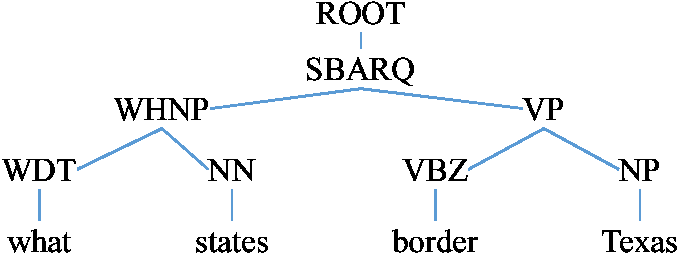
\includegraphics[width=0.48\columnwidth]{figure/rw/qa-parsing-xs.eps}}
  \hspace{1em}
  \subcaptionbox{基于PCCG的语义解析树\cite{zettlemoyer2012learning}\label{fig:rw-spt:b}}
    {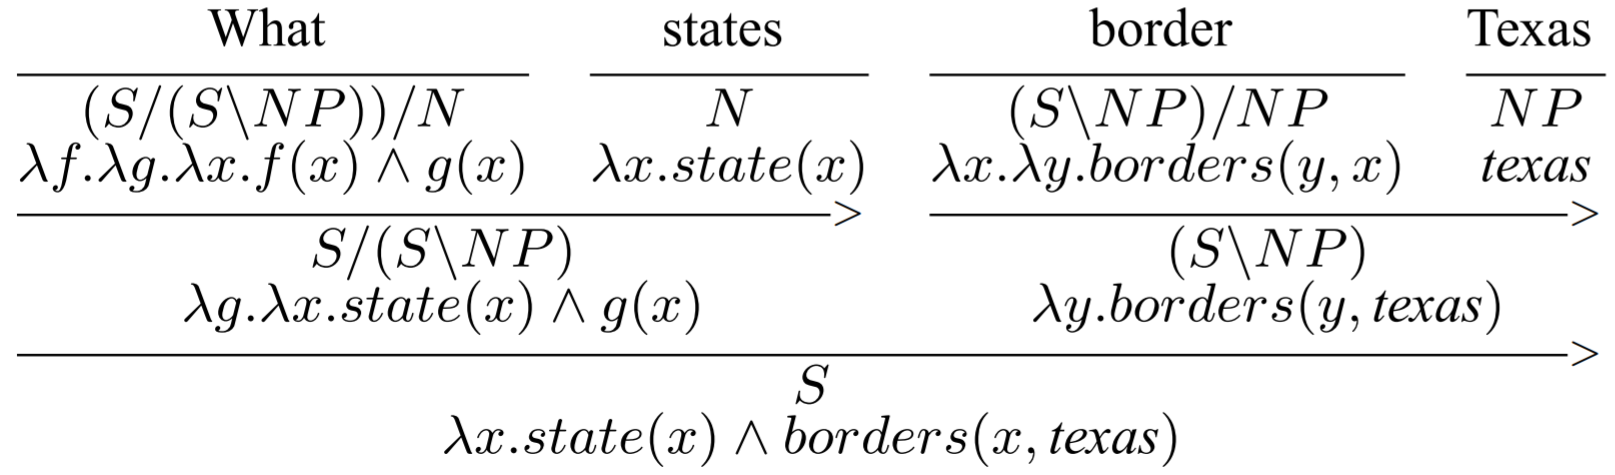
\includegraphics[width=0.48\columnwidth]{figure/rw/qa-ccg-3.png}}

  \vspace{1em}

  \subcaptionbox{基于$\lambda$-DCS的语义解析树\label{fig:rw-spt:c}}
    {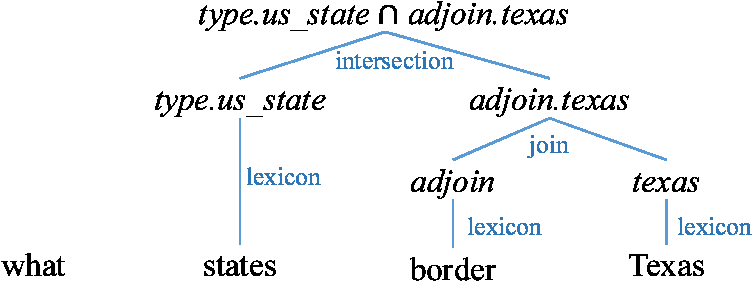
\includegraphics[width=0.48\columnwidth]{figure/rw/qa-dcs-xs.eps}}
  \hspace{3em}
  \subcaptionbox{基于多阶段生成的查询结构\label{fig:rw-spt:d}}
    {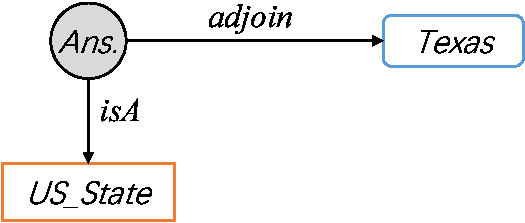
\includegraphics[width=0.38\columnwidth]{figure/rw/qa-stagg-xs.eps}}
  \bicaption{例句 ``what state borders texas'' 的多种解析结构。}
            {Several parsing structures for the question ``what state borders texas''.}
  \label{fig:rw-spt}
\end{figure}

%kwiatkowski2010inducing
%CCG cite
早期的语义解析模型\cite{zettlemoyer2012learning,kwiatkowski2010inducing,cai2013large}
使用概率化组合文法  (Probabilistic Combinatory Categorial Grammar,PCCG)
生成语义解析树。
该方法与语法解析中的概率化上下文无关文法(Probabilistic Context-Free Grammar,PCFG)相似,
根据训练数据学习文法中不同生成式规则的概率值,
并自底向上推理出每个句子最可能生成的成分解析树(Constituency Parsing Tree)。
\figref{fig:rw-spt:a}为例句的成分解析树,描述了整句的语法结构,
并标出了不同短语在句中的成分。
通过PCCG生成的语义解析树如\figref{fig:rw-spt:b}所示,
PCCG的生成式规则中不仅具有代表语法的成分信息,
同时还包含代表语义的$\lambda$表达式,
因此不同成分按照语法规则组合的过程中,
各自$\lambda$表达式也在进行拼接,从而得到对应整句话语义的逻辑表示。
PCCG语法具有很强的语义表示能力,
但由于生成式规则中涉及到不同的$\lambda$表达式,
同时训练数据匮乏,使得模型的训练具有难度。

% CCG: 语法以及语义,用lambda表达式来描述,
% 例如Inducing Probabilistic CCG Grammars from Logical Form
% with Higher-Order Unification
% 的例子,borders的那个
% 不仅语法组合成更高级的结构,语义也具有lambda表达式中的传参
% 
% PCCG: 同样概率介入,因为有多种合并方式。
% (lexicon怎么建,还要涉及词组)
% 特点:完全自底向上,每一个词都有用处(但是不是把问题搞复杂了)
% 可以支持很多操作,例如max、min、order等语义。
% 以及on-the-fly,语义解析树还需要一步转换,定位到特定的KB。


Liang在2013年提出的$\lambda$-DCS\cite{liang2013lambda}
旨在以更加简单的概念和流程,将问句转换为Freebase上的语义解析树。
如\figref{fig:rw-spt:c}所示,生成过程依然是自底向上模式,
叶节点(单词或词组)对应Freebase中的实体、类型或谓词,
但不再具有显式且复杂的$\lambda$表达式。
$\lambda$-DCS定义了节点组合过程的有限种语义合并方式,
包括连接、交集、并集甚至更加高阶的最值、计数等操作,
使得与PCCG相比,
生成的语义解析树在结构更加简单的同时,
牺牲了一定表达能力,
但对于事实类问题的理解来说依然足够。

Yih等人\cite{yih2015semantic}提出了一种多阶段的语义结构生成方法,
如\figref{fig:rw-spt:d}所示,语义解析树被表示为有向图形式,称为查询图,
图中的每一条边以及连接的两个节点,都对应\eqnref{eqn:logic-form}中的三元组。
与之前两种方法的自底向上生成不同,
多阶段语义结构生成基于由简到繁,逐步生成查询图的思路。
最简单的查询图为答案节点通过谓词(或多个谓词构成的序列)连接至
问句中的某一实体,形成仅有一条有向路径构成的查询图。
问句中抽取的其它实体、类型、时间等信息,则通过多个不同的阶段,
逐步连接至已有的路径上,构成更加复杂的查询图。
该方法不受限与问句中词的先后顺序,查询图的生成更加灵活,
在多个问答数据集上均有良好的效果。

Cui等人\cite{cui2017kbqa}提出了一种基于模板的方式,
对问句生成谓词序列形式的语义结构。
模板是对问句抽象表示,它将问句中的实体替换成类型,指代了一组具有相同语法和语义描述的问句,
``what states border \textit{\$location}'' 是一个具体的模板例子。
模板的提取依靠外部的大规模问答数据,
作者对Yahoo! Answers中大约41M问答对进行实体与答案识别后,
生成了约27M不同的模板,并通过EM算法学习其指向谓词序列的条件概率。
对于每一个问句的语义结构生成,则通过生成模型,由模板进行过渡得到不同谓词序列的概率。
这样的方法,优点在于利用大量外部数据获取准确率高的模板以及和语义的匹配,
但模型的召回率可能成为短板,当问句语法不规范时,简单的模板匹配容易失效。
%此外,其它的语义解析结构的生成方式,
%例如基于固定模板的结构生成\parencite{bast2015more,cui2017kbqa},
此外,一些文献\parencite{reddy2016transforming,hu2018answering}
使用了基于依存语法树转换的方式,利用结构相似性实现语义解析结构的生成,
这里不再一一介绍。


\subsubsection{语义匹配模型构建}    %文字1页,图0.25-0.5

由于自然语言的多义性,语义解析结构的生成结果通常都不唯一,
%因此模型需要计算问句与语义结构之间的匹配度,并根据问答数据进行训练。
%排名问题
因此需要对\textless 问句,语义解析结构 \textgreater 的匹配度进行建模,
选择最高匹配度的解析结构进行知识库上的答案查询。
%就三段,别多了
传统的语义解析模型主要基于特征工程,
Berant等人\cite{berant2013semantic}的研究工作为一个典型例子。
语义解析树由$\lambda$-DCS生成,
抽取出的特征包含三类:
问句中的短语与对应知识库谓词的对齐特征,
不同谓词参与合并的特征,
以及解析树的总体结构特征。
前两类特征来自于解析树的自底向上生成过程,用于捕捉每一个操作,
后一类特征则统计解析树中不同类型操作的数量,以及最终返回的答案数量。
%Kwai Cai Berant Bast
%基于特征工程的模型将解析树的生成看做操作序列,

为了弥补特征工程耗费人力的缺陷,同时获取更高层面的语义匹配信号,
Berant等人在后续的工作\parencite{berant2014semantic}中引入了转述特征(Paraphrasing Feature),
通过简单的规则将解析树翻译成自然语言问句,
并衡量原问句和生成问句之间是否具有转述关系,将其作为额外一组特征。
转述关系涉及到自然语言文本匹配问题,
作者使用基于词对应的关联模型和词向量的维度空间模型两种方式进行建模,
使得问答系统可以得到解析树的整体语义,是传统特征工程的有力补充。

最新的自动问答模型广泛使用了深度学习技术。
相关研究的共同点在于遵循一种 ``{编码—比较}'' 框架,
其重点在于,通过神经网络的特征学习能力,
对问句和解析结构分别进行编码,得到各自向量表示,
最后计算向量之间的相似度,代表问句与解析结构的匹配程度。
以简单问题数据集SimpQuestions为代表的问答模型几乎完全属于这一范畴,
由于在SimpleQuestions中,问句的语义解析结构均为单一谓词序列,
因此这些模型本质上都是对文本序列和谓词序列之间的匹配进行建模。
Yu等人\cite{yu2017improved}提出的HR-BiLSTM模型利用循环神经网络进行建模,
如\figref{fig:rw-siamese:a}所示,
谓词序列输入分为两个粒度:以唯一编号表示的编号序列,以及将谓词名称相连的单词序列,
分别通过双向LSTM层进行编码,
问句文本的编码也利用了双向LSTM层,并使用多层间的残差连接方式进行编码,
旨在让模型能同时捕捉单词粒度和问句整体粒度的语义信号。
SimpleQuestions上的其它类似模型还包括
文献\parencite{lukovnikov2017neural,yin2016simple,golub2016character,qu2018question}。

\begin{figure}[ht]
\centering
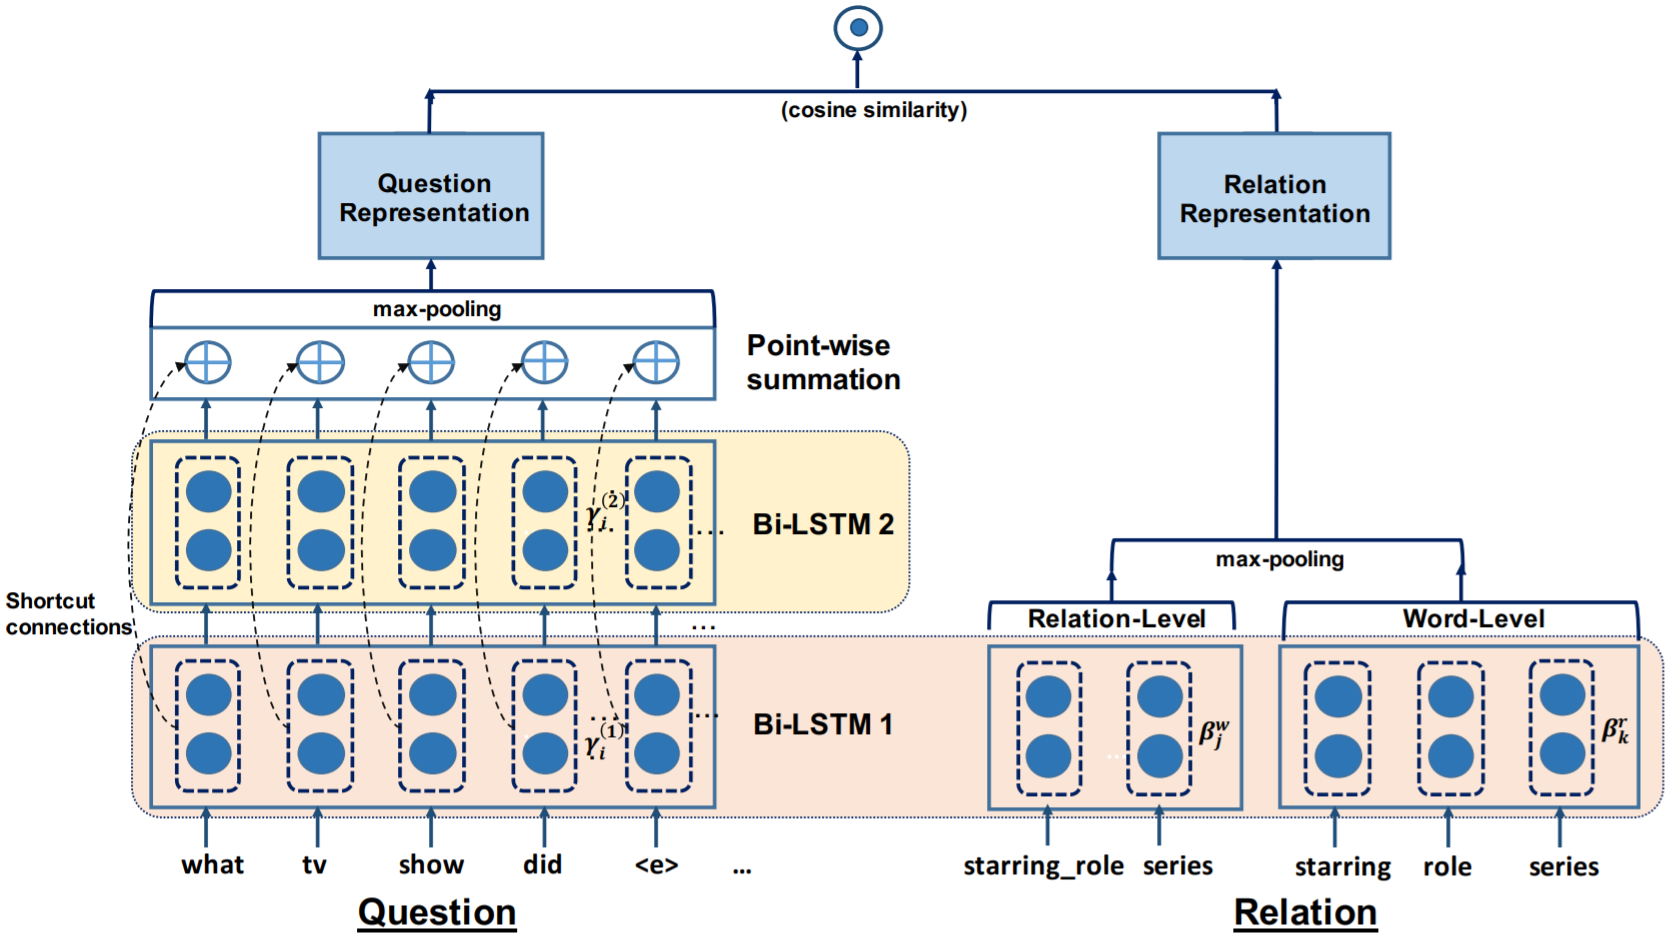
\includegraphics[width=0.95\columnwidth]{figure/rw/qa-hrbilstm.png}
\bicaption{HR-BiLSTM模型。\cite{yu2017improved}}{The HR-BiLSTM model.}
\label{fig:rw-siamese:a}
\end{figure}

对于WebQuestions等数据集上的复杂问题,如同\figref{fig:rw-spt:d}的查询图,
虽包含多条路径,但也可以选择其中最重要的路径作为主体与问句计算匹配程度。
微软的两个自动问答的研究工作\parencite{yih2015semantic,bao2016constraint}
利用了基于卷积神经网络的CDSSM匹配模型\cite{shen2014learning},
对问句和谓词路径的特征学习更多关注局部的词序信息,见\figref{fig:rw-siamese:b}。
其中,前一个研究工作由Yih等人\cite{yih2015semantic}提出,
深度学习模型仅关注问句和最重要谓词路径的匹配度,
对于查询图的其它分支路径,依然使用特征工程的方式寻找问句和谓词的字面匹配。
Bao等人\cite{bao2016constraint}的改进在于同样利用CDSSM模型,
对分支路径与问句中的特定上下文进行匹配,替代了繁琐的特征工程。
然而这些模型并没有能够学习到查询图整体在连续语义空间的特征表达,
不同路径的语义互相独立,因此面对复杂问题仍存在缺陷,这也是我们的研究重点。
%xu的先不聊
%找机会聊Hu和Cui,这两个最好还是提一提

\begin{figure}[ht]
\centering
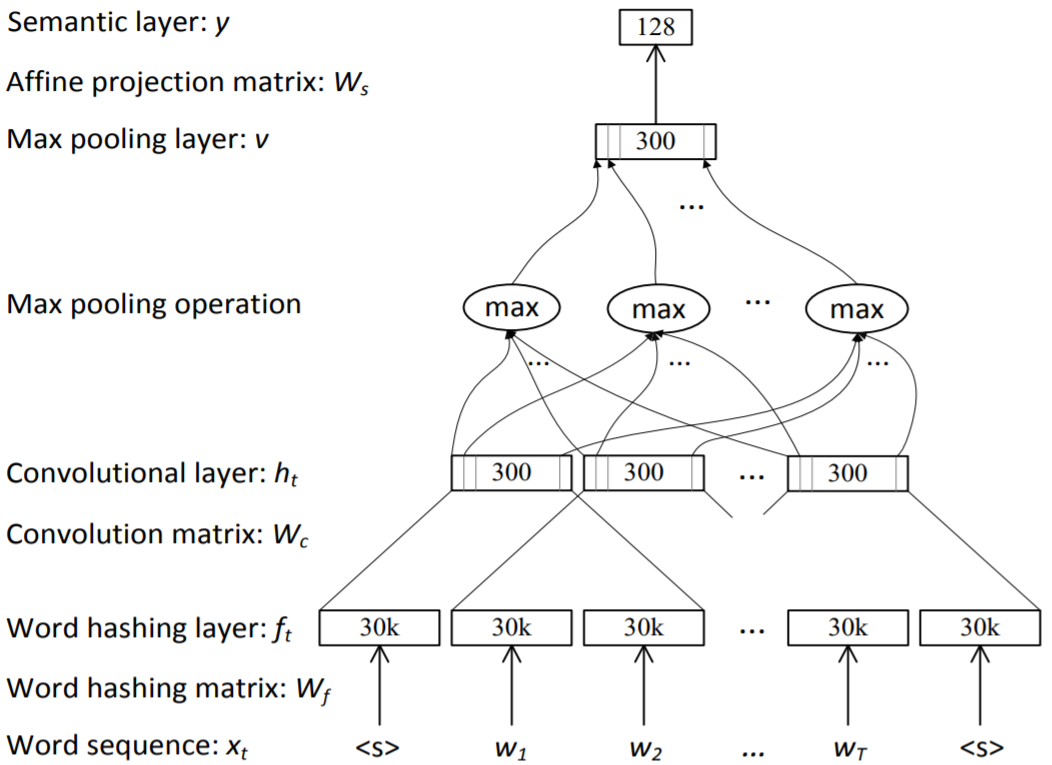
\includegraphics[width=0.6\columnwidth]{figure/rw/qa-cdssm.png}
\bicaption{CDSSM模型。\cite{shen2014learning}}{The CDSSM model.}
\label{fig:rw-siamese:b}
\end{figure}

%\begin{figure}[ht]
%  \centering
%  \subcaptionbox{HR-BiLSTM模型\cite{yu2017improved}\label{fig:rw-siamese:a}}
%    {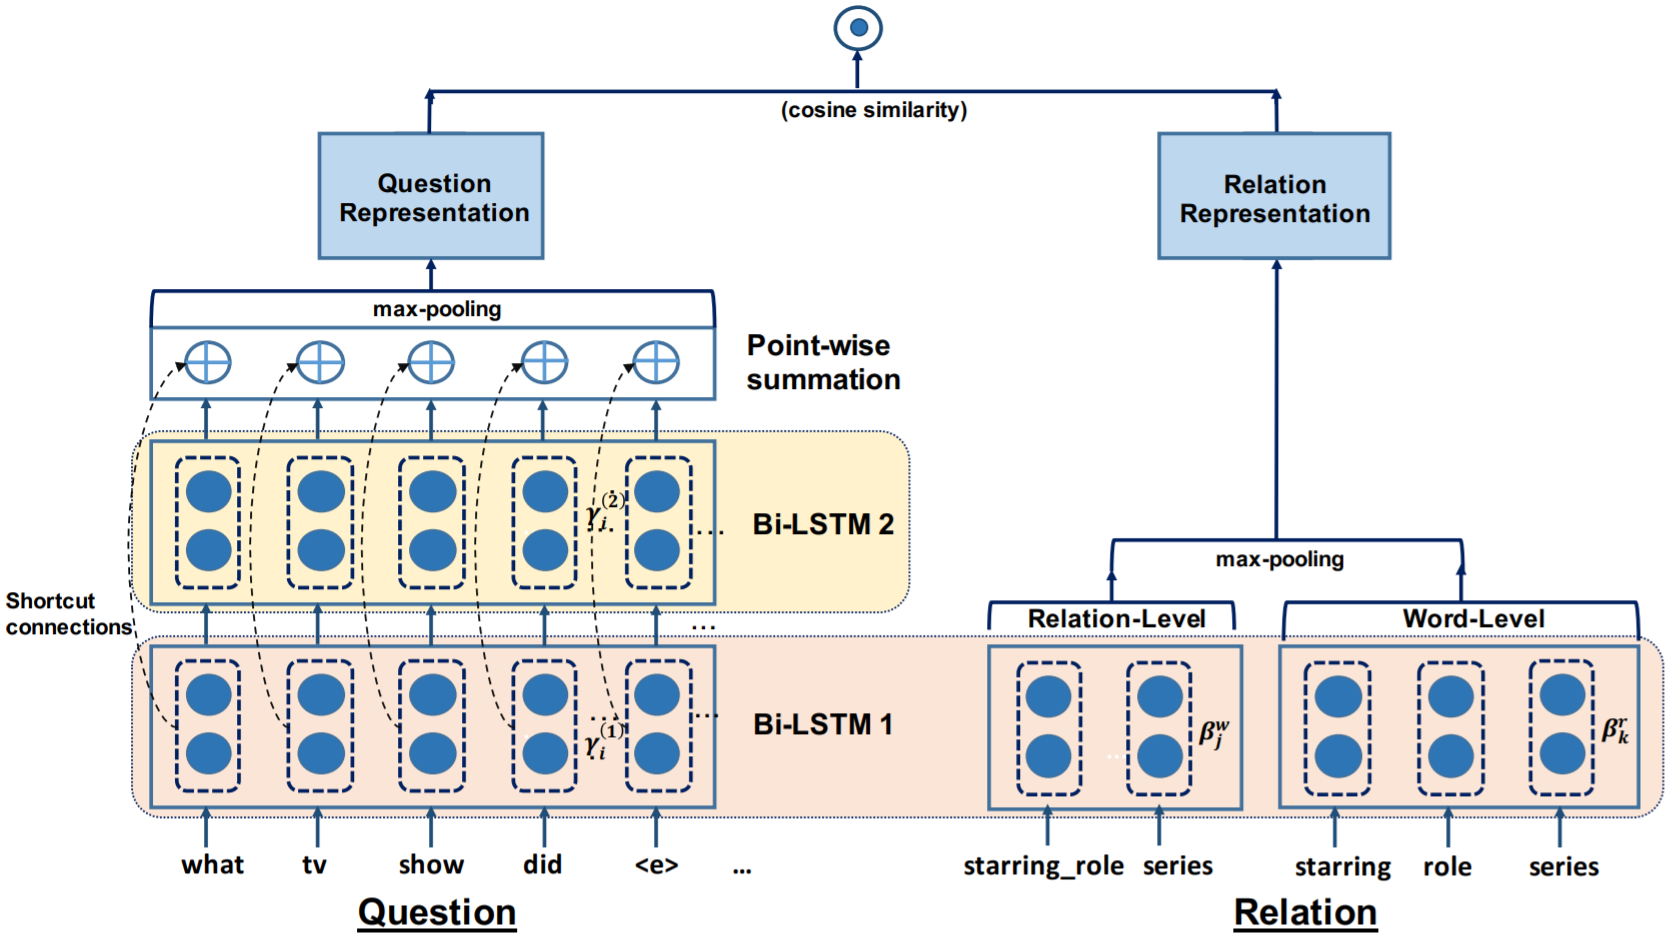
\includegraphics[width=0.48\columnwidth]{figure/rw/qa-hrbilstm.png}}
%  \hspace{1em}
%  \subcaptionbox{CDSSM模型\cite{shen2014learning}\label{fig:rw-siamese:b}}
%    {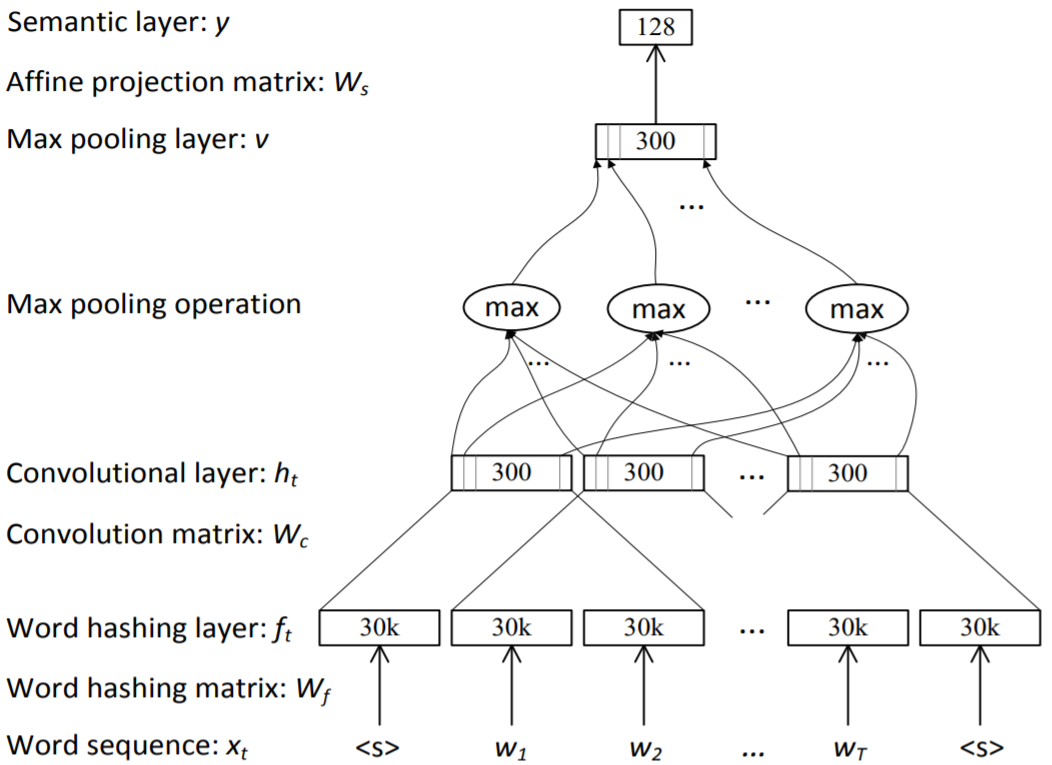
\includegraphics[width=0.48\columnwidth]{figure/rw/qa-cdssm.png}}
%
%  \bicaption{语义解析方法中,用于衡量语义匹配度的神经网络模型示例。}
%            {Example semantic matching models used in semantic parsing approaches.}
%  \label{fig:rw-siamese}
%\end{figure}

\subsubsection{训练方式}

训练方式的不同,主要取决于训练集中是否包含已标注的语义解析结构。
已有的问答数据集中,Free-917人工标注了每个问题的逻辑表达式,
QALD系列数据集则标注了SPARQL查询语句。
对于这些正确结构已给定的数据集,
可以直接利用监督学习算法进行匹配度训练。

显然语义结构的标注需要知识库领域的专家,因此标注过程会消耗大量人力,
更大规模的数据集例如WebQuestions和ComplexQuestions
仅包含每个问题的正确答案,而没有语义结构信息。
对于这些数据集,首先需要通过远距离监督方式构造可直接使用的训练数据,
即对所有训练问题,自动生成语义结构的正负样本。
已有的方法主要利用$F_1$分数衡量语义结构的好坏,
兼顾其生成的查询结果的准确率与召回率,即$F_1=2 \cdot P \cdot R / (P+R)$,
其中$P$代表准确率,$R$代表召回率。
再通过设定阈值将不同的语义结构划分为正负样本,
例如Berant等人\cite{berant2013semantic}仅将$F_1$分值为1(即答案完全匹配)
的语义结构作为正样本,
而Yih等人\cite{yih2015semantic}则将阈值设为0.5,
容忍一定程度的答案不完全匹配。
远距离监督方式避免了人工标注大量语义结构,
但考虑到语义偏差的存在,即答案正确的语义结构未必正确,
自动生成的训练数据也会引入一定量的错误。

%写类似p(g|q)之类的玩意儿刻画loss

%1. Template based (Bast, Yahya?)
%
%2. CCG (UBS, Kwai, CaiYates)
%
%3. DCS (Berant)
%
%4. Dependency Parsing Transform (Reddy, Hu)
%
%5. Staged Parsing (Yih, Bao)
%
%
%如何训练?
%
%传统Feature based (1,2,3)
%
%
%Improvements
%Berant14
%Yih
%Bao
%Xu...




\subsection{基于信息抽取的问答模型}

基于信息抽取的自动问答模型旨在直接从知识库中寻找正确答案,
而不尝试对问题进行具体化的语义建模。
模型主要包含三个步骤:
1) 对问句进行实体链接,得到其中包含的相关实体;
2) 在知识库中抽取出这些相关实体周围的其它实体,构成候选答案集合;
3) 计算问句与每一个候选答案的匹配度,以此预测出其中的正确答案实体。
显然模型的关键点在于第三步,即以怎样的特征描述候选答案与问句之间的关联。
在知识库中,一个实体所具有的信息主要包含它的名称、类型、
直接相连的谓词以及周围的其它实体。
这些信息组成了知识库中以该实体为中心的局部图,
不同的信息抽取模型都以这样的局部图作为候选答案实体的输入。
而这些模型的区别,在于特征的选取或学习方式。

Yao等人\cite{yao2014information}提出的模型利用特征工程方式,
将问句特征与候选答案特征进行配对组合,得到大规模的关联特征。
问句侧的特征来源于依存语法树,从中抽取出不同的依存路径,
以及具有强烈语义的词汇(如动词,wh-疑问词)。
答案侧的特征为答案的类型,以及与问句已知实体相连的谓词路径。
通过训练,具有高相关性的配对特征
(例如疑问词``where'' 与答案类型$location$配对)将具有更高的权重。

深度学习同样适用于基于信息抽取的问答模型。
Bordes等人\cite{bordes2014question}提出了QASE模型,
同样基于``{编码—比较}'' 框架,如\figref{fig:rw-ir:a}所示,
问句和候选答案的局部图分别进行编码,
问句的编码信息为每个词的出现次数,
候选答案则通过二进制编码表示答案实体自身、所属类型、相邻的谓词等信息。
模型学习映射矩阵$W$,将各自编码转换为连续空间上的语义向量,
$W$的每一行对应一个元素(词、实体、类型、谓词)的向量表示,
因此该模型实现了词向量和知识库向量的联合建模。

\begin{figure}[ht]
\centering
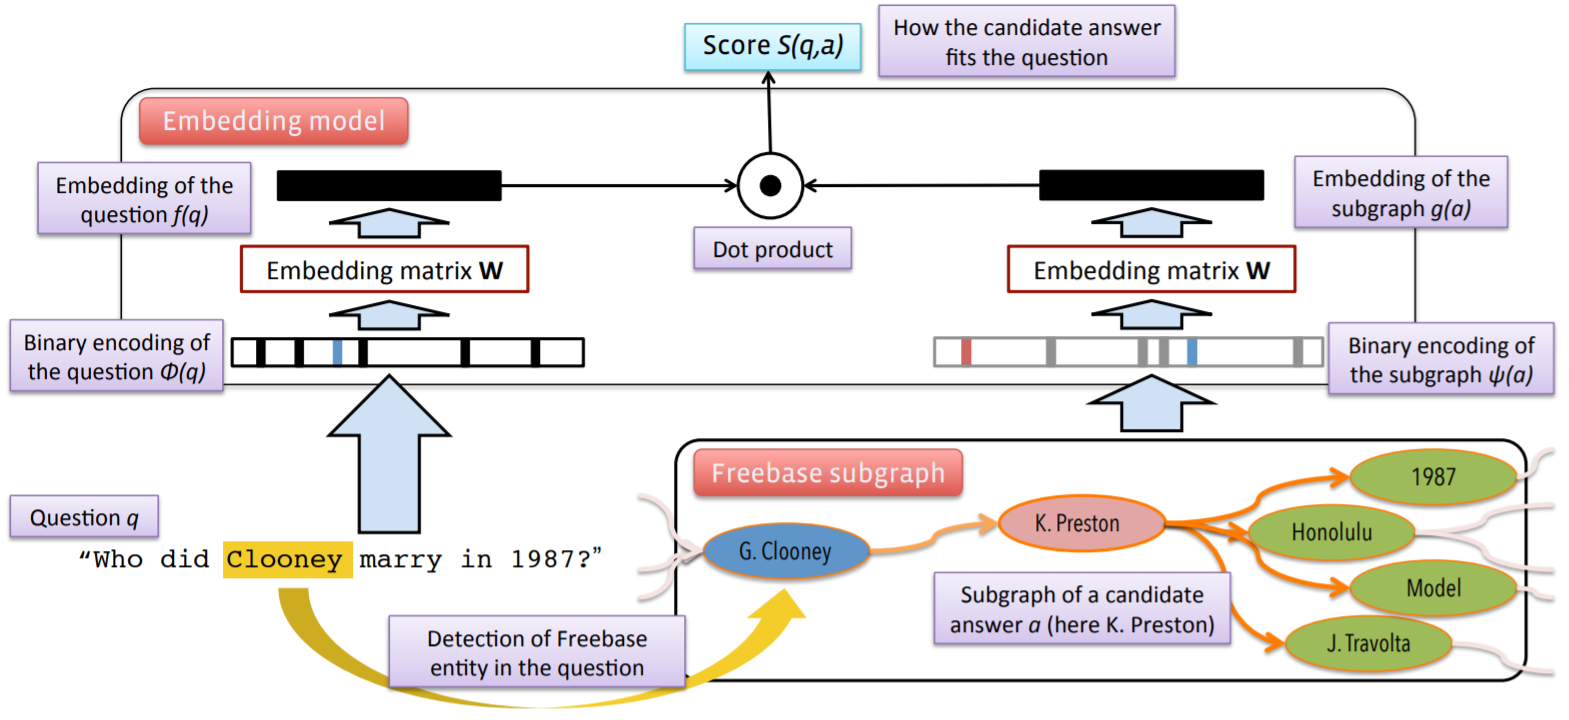
\includegraphics[width=0.95\columnwidth]{figure/rw/qa-qase.png}
\bicaption{QASE模型。\cite{bordes2014question}}{The QASE model.}
\label{fig:rw-ir:a}
\end{figure}

还有一些深度学习模型采用问句分别与答案相关的不同维度信息计算相似度,
再将各个维度的相似度进行聚合,得到问句与候选答案的整体匹配度。
Dong等人\cite{dong2015question}提出了MCCNN模型,
如\figref{fig:rw-ir:b}所示,
模型使用多个不同的卷积神经网络层对问句进行编码,
从而得到问句针对不同信息的向量表达。
将它们分别与答案的类型、谓词、上下文向量表达计算相似度之后,
最终的匹配度为这些相似度分值的总和,
使得模型在寻找最佳答案时能兼顾来自不同方面的匹配特征。

\begin{figure}[ht]
\centering
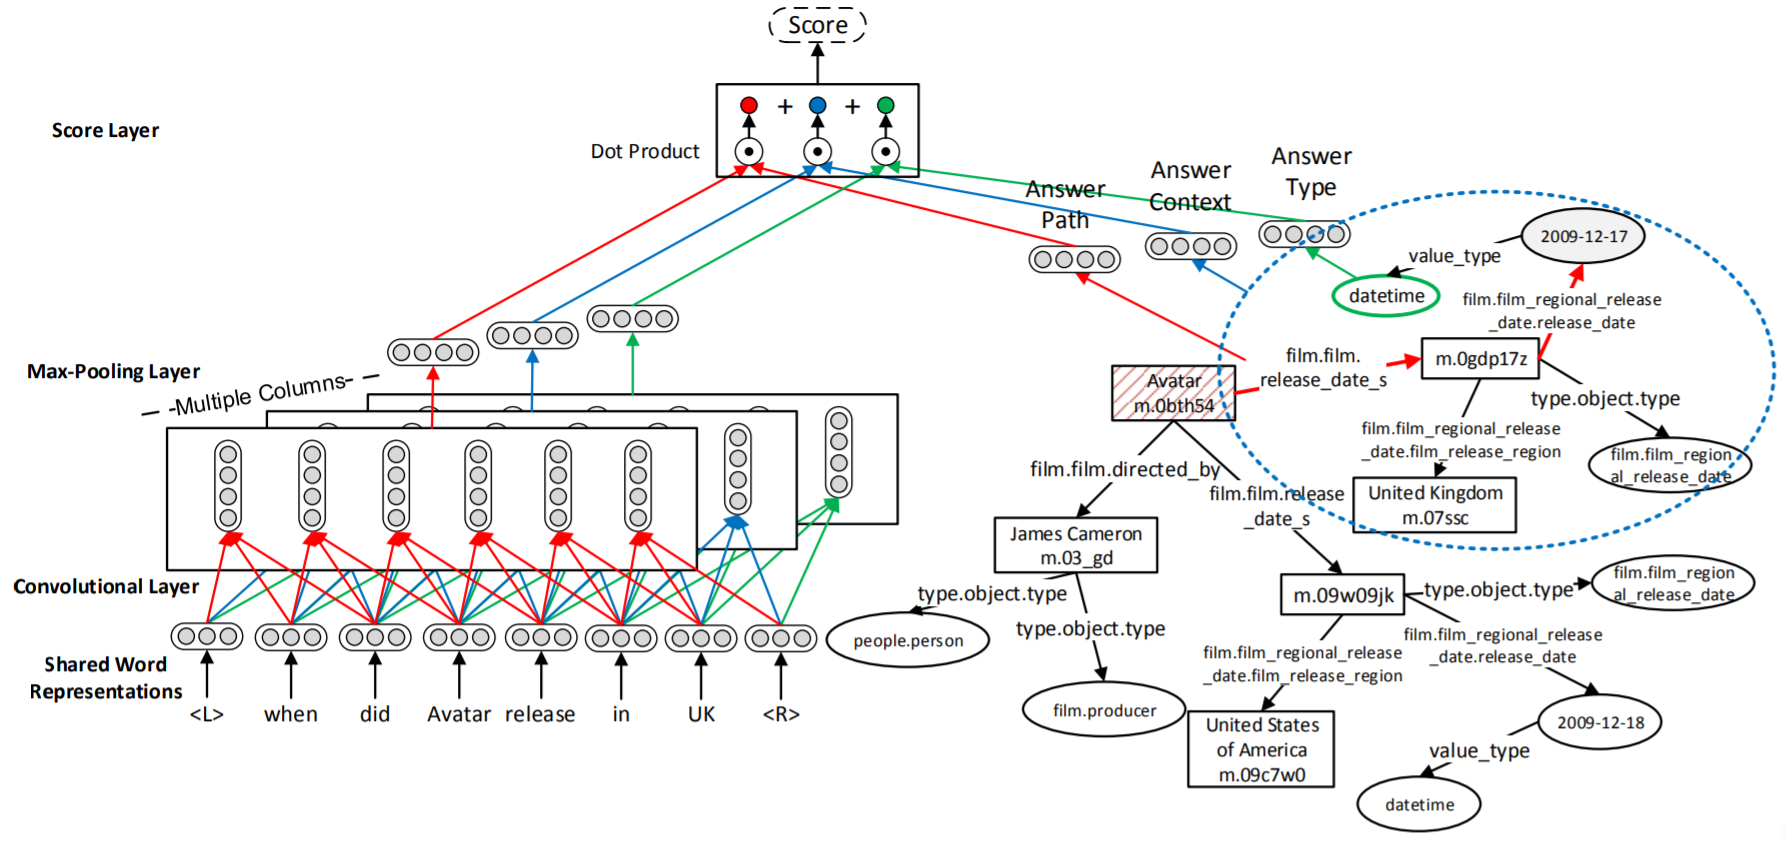
\includegraphics[width=0.95\columnwidth]{figure/rw/qa-mccnn.png}
\bicaption{MCCNN模型。\cite{dong2015question}}{The MCCNN model.}
\label{fig:rw-ir:b}
\end{figure}

Hao等人\cite{hao2017end}的模型在MCCNN基础上进行了改良,
除了将问句编码多个卷积层改为唯一一个双向LSTM层以外,
主要的贡献在于模型中使用了问句和答案之间的双向注意力机制。
一方面,针对答案在不同方面的表达,
答案对问句的注意力能够动态调整问句中不同词的重要性,
另一方面,问句对答案的注意力使得多个相似度分值互相之间也具有权重,
模型训练效果要优于无差别的求和操作。

%\begin{figure}[ht]
%  \centering
%  \subcaptionbox{QASE模型\cite{bordes2014question}\label{fig:rw-ir:a}}
%    {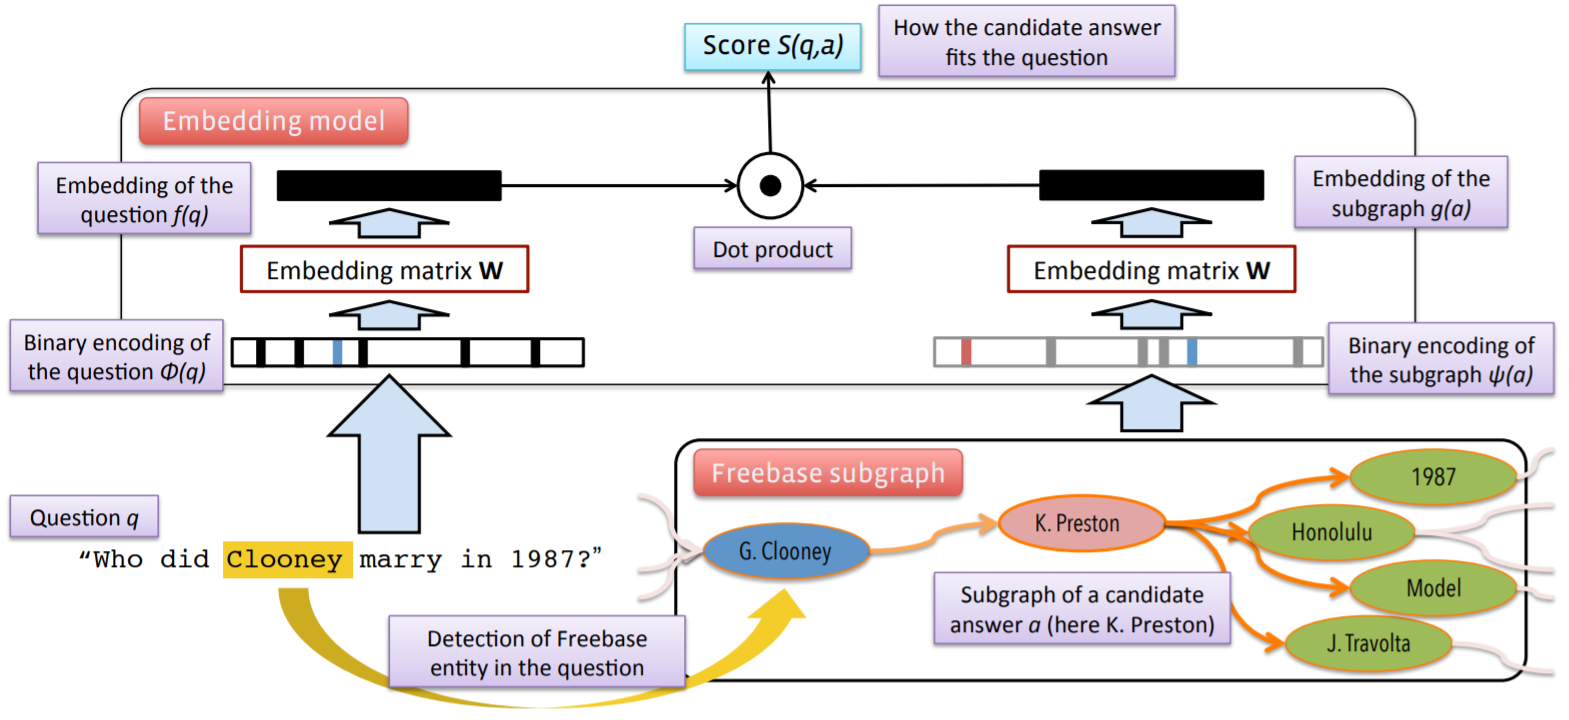
\includegraphics[width=0.48\columnwidth]{figure/rw/qa-qase.png}}
%  \hspace{1em}
%  \subcaptionbox{MCCNN模型\cite{dong2015question}\label{fig:rw-ir:b}}
%    {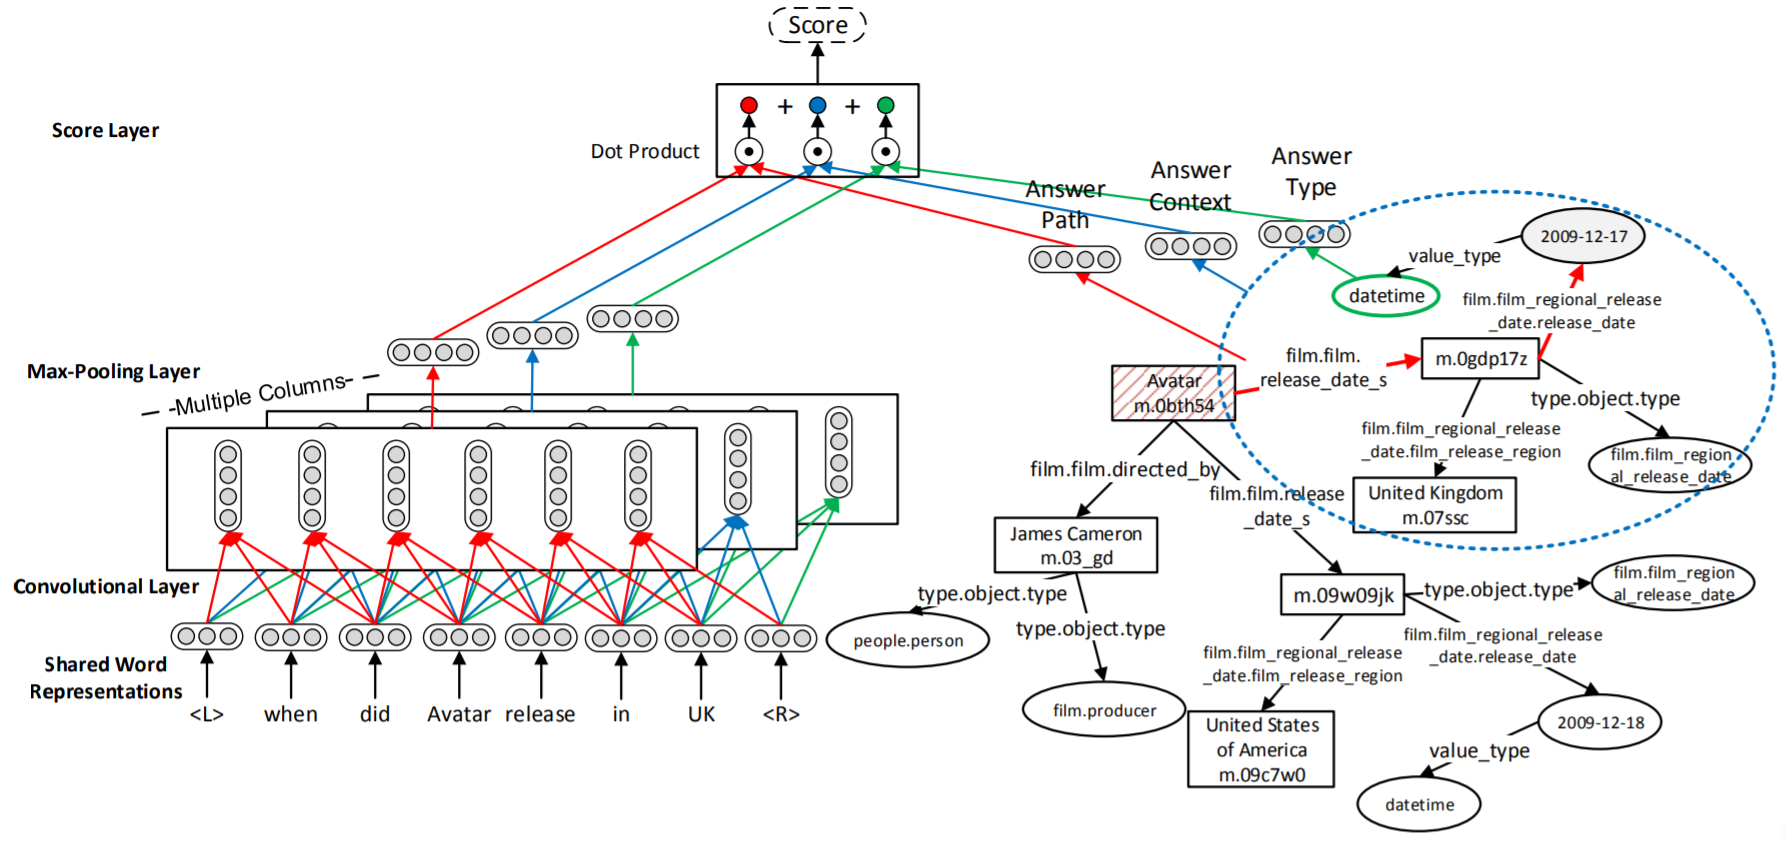
\includegraphics[width=0.48\columnwidth]{figure/rw/qa-mccnn.png}}
%
%  \bicaption{信息抽取方法中,用于衡量语义匹配度的神经网络模型示例。}
%            {Example semantic matching models used in information retrieval approaches.}
%  \label{fig:rw-ir}
%\end{figure}

和语义解析模型比较,
信息抽取模型实现了问答系统的端到端训练,
直接以\textless 问题,答案 \textgreater 作为训练数据,
防止远距离监督引入错误。
但同时也具有解释性较低的缺陷,
无法直接输出模型所理解的问句语义结构,
有时答案预测虽正确,但特征中可能存在语义偏差。
对于复杂语义的自动问答研究,
我们更在意语义结构的正确性,它能直接体现一个问答模型是否具有良好的语义理解能力。




\section{本章小结}
\label{chap:rw-summary}

本章对实体、关系、问句理解这三个层面的研究进行了背景介绍和文献综述。
实体理解方面,深度学习模型和跨语言词向量是我们较为关心的内容,
将会在第三章的跨语言表格链接任务中使用。
关系和问句理解方面,本章各介绍了两种路线不同的方法,
分别是关系理解的规则推导、知识库向量表示,
以及问句理解的语义解析、信息抽取。
这四种方法之间存在着一些共性:
规则推导和语义解析的共同点在于,
语义理解需要显式的语义结构(一阶逻辑表达式,或与之等价的知识库子图)作为媒介;
而另外两者的共同点在于对实体、类型、谓词等知识库元素进行表示学习,
以端到端的形式训练,模型更加面向具体任务。
在第四章和第五章的研究中,我们更加在意机器是否能理解具有复杂语义的关系或问句,
而不仅仅停留在特定任务的输出是否正确,
因此规则推导和语义解析是本文关注的重点。
